\documentclass[10pt,a4paper]{article}
\usepackage[utf8]{inputenc}
\usepackage[T1]{fontenc}
\usepackage[margin=1.8cm,top=2.6cm,bottom=2.2cm]{geometry}
\usepackage{parskip}
\usepackage{microtype}
\usepackage{amsmath,amssymb,mathtools}
\usepackage{array,booktabs,tabularx}
\usepackage[table]{xcolor}
\usepackage{graphicx,float}
\usepackage{titlesec}
\usepackage{enumitem}
\usepackage{fancyhdr}
\usepackage{tcolorbox}

\renewcommand\thesection{\Roman{section}}
\numberwithin{equation}{section}

\titleformat{\section}{\large\bfseries}{\thesection.\;}{0em}{}[\titlerule]
\titleformat{\subsection}{\normalsize\bfseries}{}{0em}{}
\titlespacing{\section}{0pt}{1.6ex plus .2ex}{0.6ex}
\titlespacing{\subsection}{0pt}{1.0ex}{0.3ex}

\pagestyle{fancy}
\fancyhf{}
\setlength{\headheight}{15pt}
\fancyhead[L]{\small\textit{Substrate Predictor}}
\fancyhead[R]{\small Eton iGEM Dry Lab 2026}
\fancyfoot[C]{\small\thepage}
\renewcommand{\headrulewidth}{0.35pt}

\newcommand{\cit}[1]{[#1]}
\newcommand{\FLAG}{\textit{(unconfirmed)}}
\newcommand{\CONF}{\textit{(confirmed)}}
\newcommand{\Prob}{\mathbb{P}}
\newcommand{\E}{\mathbb{E}}
\newcommand{\R}{\mathbb{R}}
\newcommand{\bm}[1]{\boldsymbol{#1}}
\newcommand{\kcat}{k_{\mathrm{cat}}}
\newcommand{\Km}{K_m}
\newcommand{\pos}[1]{\mathrm{P}#1}
\newcommand{\prm}[1]{\mathrm{P}#1'}
\newcommand{\nPosMMPtwo}{2{,}819}
\newcommand{\nNegMMPtwo}{8{,}457}
\newcommand{\aucLRMMPtwo}{0.854}
\newcommand{\aucPSSMMMPtwo}{0.874}
\newcommand{\aucConsMMPtwo}{0.869}
\newcommand{\aucLRciMMPtwo}{0.854 \,[0.844, 0.863]}
\newcommand{\aucConsciMMPtwo}{0.869 \,[0.859, 0.878]}
\newcommand{\nPosMMPeight}{698}
\newcommand{\nNegMMPeight}{2{,}094}
\newcommand{\aucLRMMPeight}{0.755}
\newcommand{\aucPSSMMMPeight}{0.784}
\newcommand{\aucConsMMPeight}{0.783}
\newcommand{\aucLRciMMPeight}{0.755 \,[0.733, 0.774]}
\newcommand{\aucConsciMMPeight}{0.783 \,[0.763, 0.800]}
\newcommand{\nPosMMPnine}{783}
\newcommand{\nNegMMPnine}{2{,}349}
\newcommand{\aucLRMMPnine}{0.760}
\newcommand{\aucPSSMMMPnine}{0.761}
\newcommand{\aucConsMMPnine}{0.772}
\newcommand{\aucLRciMMPnine}{0.760 \,[0.723, 0.791]}
\newcommand{\aucConsciMMPnine}{0.772 \,[0.737, 0.803]}
\newcommand{\nPosMMPfourteen}{717}
\newcommand{\nNegMMPfourteen}{2{,}151}
\newcommand{\aucLRMMPfourteen}{0.772}
\newcommand{\aucPSSMMMPfourteen}{0.785}
\newcommand{\aucConsMMPfourteen}{0.791}
\newcommand{\aucLRciMMPfourteen}{0.772 \,[0.753, 0.790]}
\newcommand{\aucConsciMMPfourteen}{0.791 \,[0.771, 0.810]}
\newcommand{\nPosNE}{327}
\newcommand{\nNegNE}{981}
\newcommand{\aucLRNE}{0.895}
\newcommand{\aucPSSMNE}{0.885}
\newcommand{\aucConsNE}{0.901}
\newcommand{\aucLRciNE}{0.895 \,[0.875, 0.913]}
\newcommand{\aucConsciNE}{0.901 \,[0.880, 0.919]}
\newcommand{\nPosLasB}{128}
\newcommand{\nNegLasB}{384}
\newcommand{\aucLRLasB}{0.877}
\newcommand{\aucPSSMLasB}{0.881}
\newcommand{\aucConsLasB}{0.887}
\newcommand{\aucLRciLasB}{0.877 \,[0.835, 0.917]}
\newcommand{\aucConsciLasB}{0.887 \,[0.844, 0.923]}
\newcommand{\nPosFaecal}{5{,}000}
\newcommand{\nNegFaecal}{15{,}000}
\newcommand{\aucLRFaecal}{0.951}
\newcommand{\aucPSSMFaecal}{0.953}
\newcommand{\aucConsFaecal}{0.953}
\newcommand{\aucLRciFaecal}{0.951 \,[0.948, 0.954]}
\newcommand{\aucConsciFaecal}{0.953 \,[0.950, 0.956]}
\newcommand{\rhoNElevenLR}{0.58}
\newcommand{\rhoPNElevenLR}{0.068}
\newcommand{\rhoLoNElevenLR}{-0.23}
\newcommand{\rhoHiNElevenLR}{0.93}
\newcommand{\rhoNTwelveLR}{0.68}
\newcommand{\rhoPNTwelveLR}{0.017}
\newcommand{\rhoLoNTwelveLR}{0.02}
\newcommand{\rhoHiNTwelveLR}{0.96}
\newcommand{\rhoNElevenPSSM}{0.70}
\newcommand{\rhoPNElevenPSSM}{0.020}
\newcommand{\rhoLoNElevenPSSM}{-0.00}
\newcommand{\rhoHiNElevenPSSM}{0.96}
\newcommand{\rhoNTwelvePSSM}{0.75}
\newcommand{\rhoPNTwelvePSSM}{0.006}
\newcommand{\rhoLoNTwelvePSSM}{0.18}
\newcommand{\rhoHiNTwelvePSSM}{0.93}
\newcommand{\rhoNElevenCons}{0.57}
\newcommand{\rhoPNElevenCons}{0.074}
\newcommand{\rhoLoNElevenCons}{-0.21}
\newcommand{\rhoHiNElevenCons}{0.90}
\newcommand{\rhoNTwelveCons}{0.66}
\newcommand{\rhoPNTwelveCons}{0.021}
\newcommand{\rhoLoNTwelveCons}{0.06}
\newcommand{\rhoHiNTwelveCons}{0.91}
\newcommand{\mutOneMeasured}{1.25}
\newcommand{\mutOneLR}{1.63}
\newcommand{\mutOnePSSM}{1.99}
\newcommand{\mutTwoMeasured}{-5.08}
\newcommand{\mutTwoLR}{-0.21}
\newcommand{\mutTwoPSSM}{-1.31}
\newcommand{\maxLeakGap}{0.007}
\newcommand{\shuffleMin}{0.49}
\newcommand{\shuffleMax}{0.53}
\newcommand{\subspaceMin}{64}
\newcommand{\subspaceMax}{79}
\newcommand{\pssmRankPThreePro}{1}
\newcommand{\pssmLOPThreePro}{+2.80}
\newcommand{\pssmRankPTwoArg}{4}
\newcommand{\pssmLOPTwoArg}{+0.35}
\newcommand{\pssmRankPOneThr}{16}
\newcommand{\pssmLOPOneThr}{-1.14}
\newcommand{\pssmRankPOneSer}{9}
\newcommand{\pssmLOPOneSer}{-0.18}
\newcommand{\pssmRankPOnePLeu}{1}
\newcommand{\pssmLOPOnePLeu}{+1.36}
\newcommand{\pssmRankPOnePIle}{2}
\newcommand{\pssmLOPOnePIle}{+0.85}
\newcommand{\pssmRankPTwoPSer}{18}
\newcommand{\pssmLOPTwoPSer}{-0.70}
\newcommand{\pssmRankPTwoPThr}{7}
\newcommand{\pssmLOPTwoPThr}{+0.19}
\newcommand{\pssmRankPOneGly}{1}
\newcommand{\pssmLOPOneGly}{+1.39}
\newcommand{\pssmRankPOneLys}{2}
\newcommand{\pssmLOPOneLys}{+1.25}
\newcommand{\pssmRankPOneArg}{3}
\newcommand{\pssmLOPOneArg}{+0.87}


\newenvironment{assump}{%
  \small}{%
  \smallskip}

\begin{document}

\begin{center}
{\LARGE\bfseries Substrate Predictor}\\[0.4em]
{\large How a P4--P4$'$ Substrate Window Becomes a Panel Selectivity Score}\\[0.25em]
{\small\color{gray}
Eton iGEM 2026, Dry Lab \quad$|$\quad
Tasks 7 and 8 \quad$|$\quad
\texttt{spred} package}
\end{center}
\vspace{0.4em}\hrule\vspace{0.7em}

\noindent\textbf{Scope.}
This document presents the software tool that scores an eight-residue
peptide window against a panel of proteases, the methodology by which its
models were built and evaluated, and the extent to which its outputs can be
relied upon. It is organised into six sections, each corresponding to one
stage from source data to design decision. Each section follows a
consistent structure: a plain-language description of the stage; the
assumptions required for the stated result, given explicitly; the governing
equations; and the resulting evidence. Values obtained by direct computation, or verified
against a source held in the repository, are annotated \CONF. Values that
represent a working assumption, or that could not be checked
independently, are annotated \FLAG.

%=======================================================================
\section{Overview: Model Structure and Operating Principle}
\label{sec:story}

A protease hydrolyses one peptide bond, the \emph{scissile bond}. Residues
on its amino-terminal side are numbered outward from the bond as
$\pos{1},\pos{2},\dots$ and residues on the carboxy-terminal side as
$\prm{1},\prm{2},\dots$ \cit{1}. The enzyme surface that receives residue
$\pos{i}$ is subsite S$i$, and $\prm{i}$ binds S$i'$. Specificity is
therefore positional: a protease may require proline at $\pos{3}$ and a large
hydrophobic residue at $\prm{1}$, and these preferences are largely
independent of one another. The unit of data throughout this document is the
eight-residue window
\[
\underbrace{\pos{4}\ \pos{3}\ \pos{2}\ \pos{1}}_{\text{non-primed}}\ \ \downarrow\ \ \underbrace{\prm{1}\ \prm{2}\ \prm{3}\ \prm{4}}_{\text{primed}},
\]
so that the scissile bond always lies between the fourth and fifth character.
For example, the MMP-9 substrate SGKIPRT$\downarrow$LTA measured by
Kridel et al.\ \cit{1} has $\pos{4}\pos{3}\pos{2}\pos{1}=\mathrm{IPRT}$ and
$\prm{1}\prm{2}\prm{3}=\mathrm{LTA}$; its window is \texttt{IPRTLTA}$-$, with
$\prm{4}$ unknown because the peptide ends there.

The panel comprises the matrix metalloproteinases MMP-2, MMP-8, MMP-9 and
MMP-14, neutrophil elastase (NE), LasB (pseudolysin of \emph{Pseudomonas
aeruginosa}), and a pooled group of digestive serine proteases (trypsin~1,
chymotrypsin~B and elastase-1; MEROPS S01.151--153), giving seven
trainable proteases and $10{,}472$ confirmed cleavage windows \CONF. The MMPs
are zinc-dependent endopeptidases whose catalytic domain of about 170
residues carries the zinc-binding motif HEXXHXXGXXH and a conserved
methionine (the ``Met-turn''), together with a structural zinc and two to
three calcium ions \cit{2}. MMP-9 substrates selected by phage display
carry Pro at $\pos{3}$ and a large hydrophobic residue at $\prm{1}$, with
Arg favoured at $\pos{2}$ and Ser/Thr at $\prm{2}$; the same authors note
that many MMPs recognise this Pro-X-X-Hy core and that selectivity must
therefore arise from subsite interactions outside $\pos{3}$ and $\prm{1}$
\cit{1}. MMPs are reported to be elevated in chronic wound fluid relative to
acute wound fluid, with MMP-9 the predominant elevated gelatinase, while the
evidence for neutrophil elastase is mixed \cit{3}.

The tool produces, for each protease in a chosen panel, (i) a cleavage
score from a logistic regression on physicochemical features, (ii) a score
from a position-specific scoring matrix (PSSM), (iii) each score expressed as
a percentile of random background windows, so that different proteases are
comparable, and (iv) a specificity margin: the target's consensus percentile
minus that of its strongest competitor. The remainder of this document is
organised into six sections, each addressing one stage:
\begin{center}
\small
\begin{tabular}{@{}cll@{}}
\toprule
Part & Content & Section \\
\midrule
A & Confirmed cleavage windows and negative sets & \ref{sec:data} \\
B & Feature representation and per-protease models & \ref{sec:models} \\
C & Percentile scale and panel selectivity & \ref{sec:panel} \\
D & Evaluation methodology and cross-validated results & \ref{sec:eval} \\
E & Validation against independent data and structures & \ref{sec:valid} \\
F & Application to sensor candidate design & \ref{sec:design} \\
\bottomrule
\end{tabular}
\end{center}

\begin{figure}[H]
  \centering
  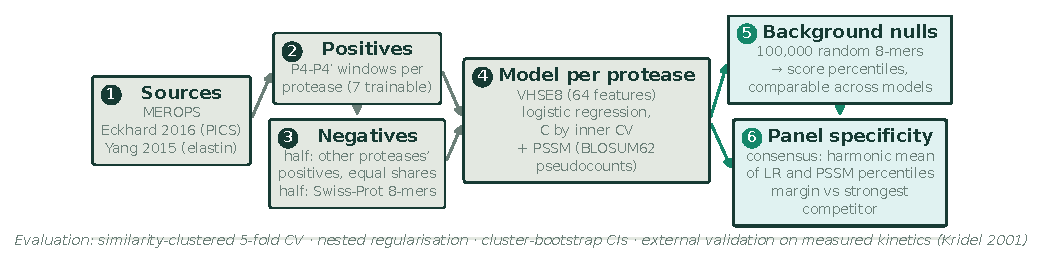
\includegraphics[width=\textwidth]{../figures/F01_pipeline.pdf}
  \caption{Pipeline from source data to panel selectivity. Positives are
    confirmed cleavage windows; negatives combine other proteases' windows
    with random background windows; each protease receives a logistic
    regression and a PSSM; scores are converted to percentiles of a
    background null and combined into a consensus and a specificity margin.}
  \label{fig:pipeline}
\end{figure}

An interactive browser version of the tool accompanies this document
(\texttt{substrate\_predictor\_explorer.html}); it embeds the trained models,
the protease structures used in Part~\ref{sec:valid}, and a scoring engine
verified against the Python package (Part~\ref{sec:design}).

%=======================================================================
\section{Part A: The Training Data}
\label{sec:data}

\subsection{Overview}

Each protease model is trained on confirmed cleavage windows. Three
sources contribute: the MEROPS \texttt{Substrate\_search} table \cit{8},
which lists for each recorded cleavage the eight residues around the
scissile bond; the proteomic identification of cleavage sites (PICS) data of
Eckhard et al.\ \cit{4} for MMP-2, MMP-8, MMP-9 and MMP-14; and the elastin
digestion data of Yang et al.\ \cit{5} for LasB. In PICS, an MMP is incubated
with peptide libraries derived from a human proteome digested with trypsin or
GluC, and cleavage products are identified by LC-MS/MS at a false-discovery
rate of 1\%; the non-primed residues $\pos{4}$--$\pos{1}$ are recovered by
locating each identified peptide in its source protein sequence. The Yang et
al.\ study identified peptides released from bovine elastin by pseudolysin by
mass spectrometry, and both termini of each released peptide are cleavage
sites.

\subsection{Assumptions}

\begin{assump}
\begin{itemize}[leftmargin=*,noitemsep]
\item \textbf{Confirmed windows are correct positives.} Windows are taken as
  recorded in the sources. The MEROPS table mixes physiological and synthetic
  substrates \FLAG.
\item \textbf{Negatives are unlabelled, not confirmed.} No window is known
  to be uncleaved; random background windows are assumed to be negatives.
  The resulting label noise is bounded in Part~\ref{sec:eval} but its
  magnitude is unknown \FLAG.
\item \textbf{Sources are pooled without correction for source bias.} PICS
  libraries are generated with trypsin or GluC, which constrains composition
  at peptide ends and may leak into primed positions of short peptides
  \FLAG.
\item \textbf{The LasB set is dominated by one protein.} $97$ of $128$
  positives ($76\%$) are windows from bovine elastin \CONF.
\item \textbf{The faecal group is heterogeneous.} It pools three
  unrelated digestive proteases (bovine trypsin~1, human chymotrypsin~B,
  porcine elastase-1) \CONF; its windows are capped at $5{,}000$ of $18{,}251$.
\end{itemize}
\end{assump}

\subsection{Sources and extraction}

MEROPS windows are read from columns $5$--$12$ of the substrate table
(three-letter code for $\pos{4}$ to $\prm{4}$), keyed by the peptidase
identifier in column~2. The Eckhard windows were extracted once from the
supplementary tables and archived; all peptides in the eight source sheets
used carry an N-terminal label ($3{,}536$ thioacyl at $+89.01$~Da and $815$ at
$+29.04$~Da, the latter not defined in the source legend) \CONF. The Yang et
al.\ Supplementary Table~S1 was re-extracted directly from the supplementary
PDF: all $75$ peptide rows were recovered, and for each row the peptide sits at
its stated position in the UniProt sequence of bovine tropoelastin (P04985)
and both flanking residues match, in all $75$ rows \CONF. The $\pos{4}$--$\prm{4}$
window is then read from that sequence around both termini of each peptide.
Rebuilding the MEROPS and Eckhard positive sets from the raw files reproduces
the counts obtained by the earlier implementation exactly \CONF.

\begin{center}
\small\renewcommand{\arraystretch}{1.25}
\begin{tabular}{@{}lrrrr@{}}\toprule
Protease & MEROPS & Eckhard 2016 & Yang 2015 & Total \\\midrule
MMP-2 & 2{,}318 & 501 & 0 & 2{,}819 \\
MMP-8 & 96 & 602 & 0 & 698 \\
MMP-9 & 341 & 442 & 0 & 783 \\
MMP-14 & 129 & 588 & 0 & 717 \\
Neutrophil elastase & 327 & 0 & 0 & 327 \\
LasB & 31 & 0 & 97 & 128 \\
Faecal serine proteases & 5{,}000 & 0 & 0 & 5{,}000 \\
\bottomrule\end{tabular}

\end{center}

The table lists positive windows per protease and source after removal of
duplicate windows; a window reported by several sources is counted once, under
the first.

\subsection{Negative sets}

For a target $t$ with $n_t$ positives the training set contains
$N=3n_t$ negatives. With $K-1=6$ competitor proteases, a quota
$q=\lfloor N/2/(K-1)\rfloor$ of windows is drawn without replacement from each
competitor's positives, excluding any window that is a positive of $t$. The
remaining negatives are random background windows whose residues are drawn
independently from the UniProtKB/Swiss-Prot amino-acid composition (release
2026\_03) \cit{10}, again excluding known positives. For MMP-9, $N=2{,}349$:
$195$ windows from each of five competitors, $121$ from LasB (its entire
eligible pool), and $1{,}253$ background windows. Construction is seeded and
reproducible. Two alternatives are evaluated in Part~\ref{sec:eval}:
background-only negatives, and the design of the earlier implementation,
composition-shuffled positives plus background.

\subsection{Near-duplicate structure}

Sequence data of this kind contain families of near-identical windows
(collagen and elastin repeats, overlapping peptides from one protein, the same
site reported by two sources). If such windows are divided between training and
test folds, a model can score well by recalling a neighbour. A graph is
therefore defined on all training windows in which two windows are adjacent
when their Hamming distance is at most $2$ (at least $6$ of $8$ residues
identical), and its connected components are termed clusters. The fraction of
each positive set with a near-duplicate ranges from $2\%$ (NE) to $28\%$
(LasB); MMP-9 contains a single cluster of $86$ windows \CONF.

\begin{figure}[H]
  \centering
  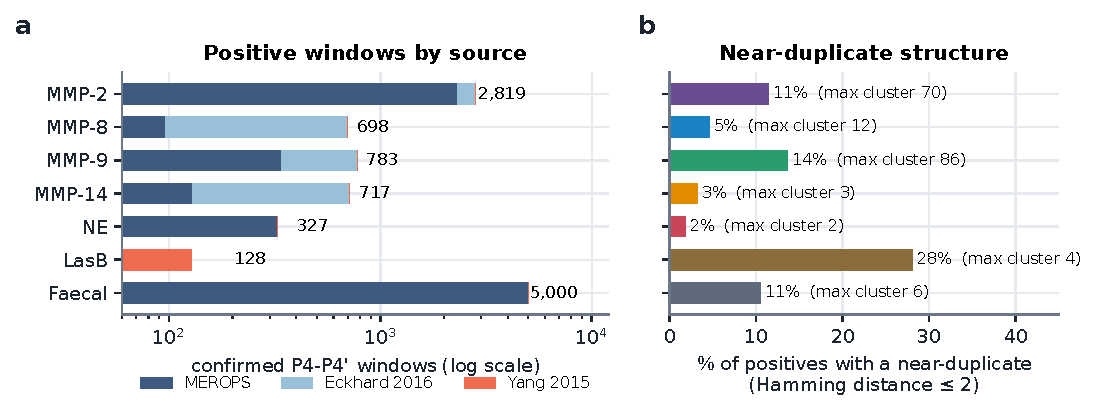
\includegraphics[width=\textwidth]{../figures/F02_data_composition.pdf}
  \caption{\textbf{A:} positive windows per protease by source (log scale).
    \textbf{B:} fraction of positives that have at least one near-duplicate
    (Hamming distance $\le2$) and the size of the largest cluster.}
  \label{fig:data}
\end{figure}

\subsection{Similarity between proteases}

Exact window overlap between protease positive sets is small (maximum Jaccard
index $0.145$, between MMP-8 and MMP-9), and windows shared with the target are
removed from its negatives. The position-specific preferences nevertheless
overlap strongly among the MMPs: the PSSM log-odds vectors of MMP-2, MMP-8 and
MMP-14 correlate at $r=0.73$--$0.82$, and MMP-9 correlates at $0.56$--$0.63$ with
each. NE is essentially uncorrelated with the MMPs and correlates with the
faecal group at $0.46$, both being serine proteases. This structure predicts
the selectivity results of Part~\ref{sec:eval}.

\begin{figure}[H]
  \centering
  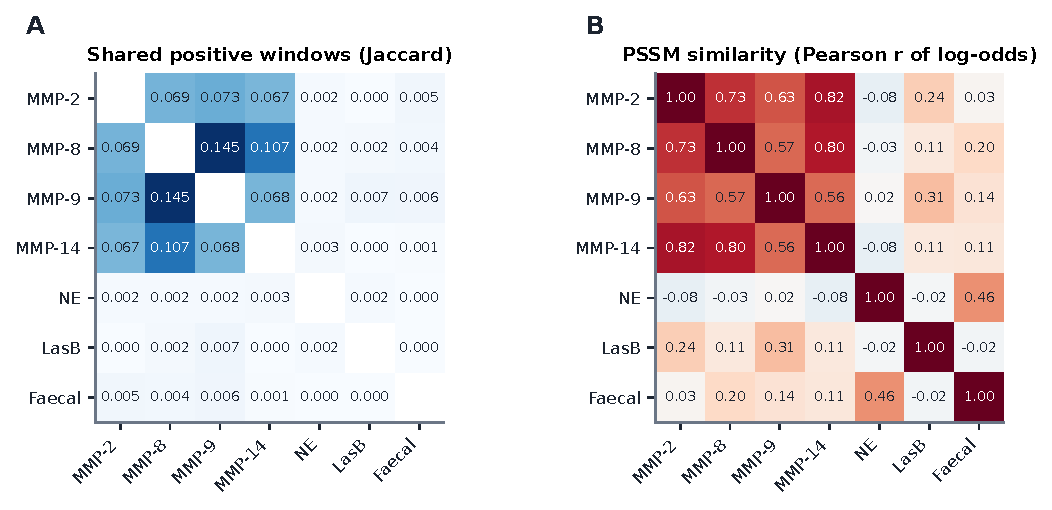
\includegraphics[width=\textwidth]{../figures/F04_protease_similarity.pdf}
  \caption{\textbf{A:} Jaccard index of exact positive windows.
    \textbf{B:} Pearson correlation of the $8\times20$ PSSM log-odds between
    protease pairs.}
  \label{fig:sim}
\end{figure}

\begin{figure}[H]
  \centering
  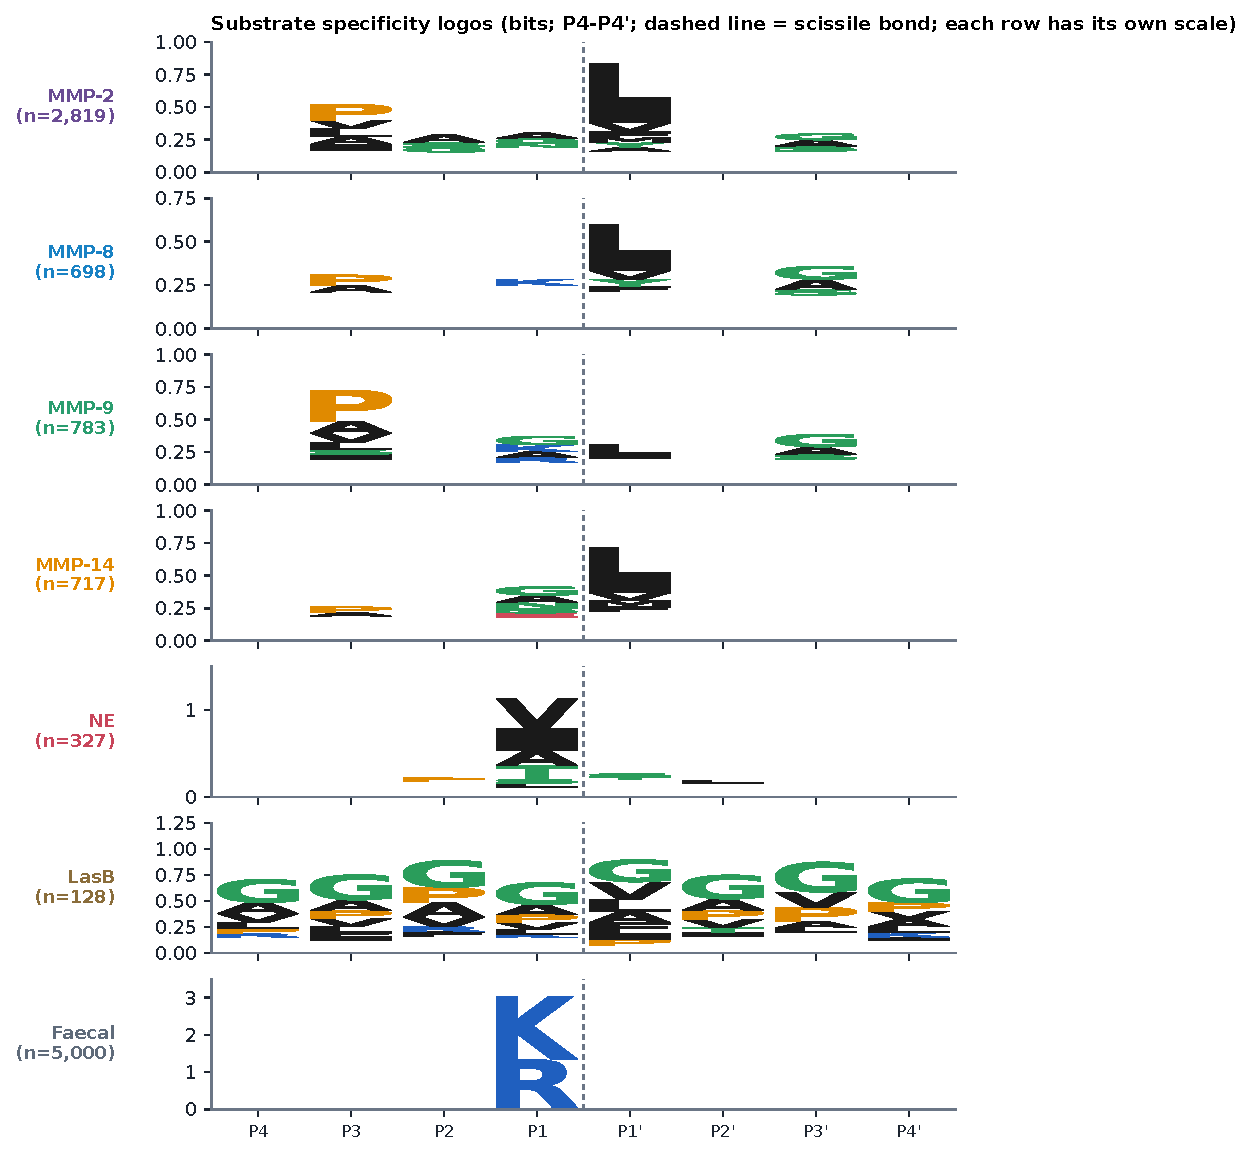
\includegraphics[width=0.86\textwidth]{../figures/F03_sequence_logos.pdf}
  \caption{Specificity logos computed from each model's PSSM (letter height is
    probability times information content; each row has its own vertical scale,
    since the MMPs carry under one bit per position while the faecal group
    exceeds three at $\pos{1}$). The MMPs share Pro at $\pos{3}$ and a
    hydrophobic residue at $\prm{1}$; NE prefers small aliphatic residues at
    $\pos{1}$; the faecal group is dominated by Lys/Arg at $\pos{1}$. The LasB
    logo is Gly-rich because $76\%$ of its positives derive from elastin.}
  \label{fig:logos}
\end{figure}

\subsection{Provenance checks and corrections}

Before the present models were built, each element of an earlier
implementation was tested with code (audit run at repository commit
\texttt{68e3dc2}; outputs retained in \texttt{results/legacy\_audit/}). The
findings, and the resulting action, are as follows.

\begin{center}
\footnotesize\renewcommand{\arraystretch}{1.2}
\begin{tabular}{@{}p{0.17\textwidth}p{0.47\textwidth}p{0.28\textwidth}@{}}
\toprule
Element & Finding & Action \\
\midrule
VHSE descriptor table & $35$ of $160$ values differed from the archived published table (several with opposite sign); glycine had been set to an all-zero reference vector, which is incorrect; descriptor labels contradicted the source definition (hydrophobic, steric, electronic); the citation named the wrong journal. Correction changed random-fold AUROC by $-0.006$ to $+0.012$. & Table regenerated from the archived file and unit-tested against it. \\
Swiss-Prot background & Two different frequency tables were in use (a residue frequency differed by up to $0.0049$). & One table from release 2026\_03. \\
Grouped cross-validation & Reported as $0.5$ for every protease: the groups were the labels positive, cross and background, so every held-out group contained one class and the function returned a fixed fallback. & Replaced by cluster-aware folds. \\
PSSM performance & Scored on the positives used to build the PSSM. In-sample versus out-of-fold AUROC: LasB $0.977$ versus $0.779$, NE $0.883$ versus $0.829$, MMP-8 $0.875$ versus $0.849$, MMP-9 $0.816$ versus $0.790$. & PSSM refit and scored out-of-fold in every fold. \\
Selectivity index & The ratio $p_t/\max p_j$ compared probabilities from models whose mean score on random windows ranged from $0.106$ to $0.328$; the median index of the top $1\%$ of MMP-9 candidates was $0.975$. & Percentile scale and margin (Part~\ref{sec:panel}). \\
LasB training data & $92$ positives were generated by a rule (every Ala$|$Ala, Val$|$Ala, Ala$|$Gly and Gly$|$Ala bond in a hard-coded elastin string) and attributed to a paper not held; $14$ more were typed by hand; four windows tagged as MEROPS were absent from the MEROPS file. None is a measured cleavage site. & Removed. LasB uses $31$ MEROPS windows and $97$ from Yang et al. \\
Elastin table & Typed by hand from the PDF; four of $75$ rows did not appear in the source. & Re-extracted from the PDF; $75$ of $75$ rows verified. \\
Kinetic table & The competing enzymes were labelled MMP-1 and MMP-2; the source gives MMP-13 and MMP-7. One measured non-substrate (C11) was omitted. & Re-extracted from the source table. \\
Report and code drift & Positive counts in the earlier report (MMP-14 $129$, MMP-8 $96$, MMP-9 $341$) no longer matched the data ($717$, $698$, $783$); a unit test asserted the incorrect glycine claim; oversampling was applied before cross-validation. & Report rewritten; test corrected; oversampling removed. \\
Model sprawl & Separate model files and scripts per experiment overwrote one another. & One model per protease. \\
\bottomrule
\end{tabular}
\end{center}

\subsection{Result}

The corrected data layer yields seven trainable proteases with
$2{,}819$ (MMP-2), $698$ (MMP-8), $783$ (MMP-9), $717$ (MMP-14), $327$ (NE),
$128$ (LasB) and $5{,}000$ (faecal group) confirmed windows. FAP is registered
but has only two confirmed windows in MEROPS and cannot be trained.

%=======================================================================
\section{Part B: Feature Representation and Models}
\label{sec:models}

\subsection{Overview}

Each protease receives two scorers. The first is a logistic regression on a
64-feature physicochemical encoding of the window; the second is a PSSM with
BLOSUM62-derived pseudocounts. Both are additive over the eight positions,
which matches the positional nature of subsite specificity, and both can
therefore be decomposed exactly into one contribution per position. The
physicochemical encoding uses the VHSE descriptors of Mei et al.\ \cit{6}:
eight principal-component score vectors derived from independent families of
$18$ hydrophobic, $17$ steric and $15$ electronic properties, of which
VHSE1--2 are hydrophobic, VHSE3--4 steric and VHSE5--8 electronic. The
descriptor table is archived with its source and unit-tested against it.

\subsection{Assumptions}

\begin{assump}
\begin{itemize}[leftmargin=*,noitemsep]
\item \textbf{Position-specific effects are additive.} The effect of a residue
  at one position is independent of the residues elsewhere in the window.
  Gradient-boosted trees, which can represent interactions, do not exceed the
  additive models by more than $0.007$ AUROC on any protease (Part~\ref{sec:eval})
  \CONF.
\item \textbf{The eight VHSE descriptors capture the relevant residue
  properties.} They express $\subspaceMin$--$\subspaceMax\%$ of the learned
  per-position specificity, depending on the protease; the remainder is
  approximation bias \CONF.
\item \textbf{The PSSM smoothing parameters are fixed.} The pseudocount weight
  $\beta=5$ and the background mixing weight $\epsilon=0.05$ were not tuned
  \FLAG.
\item \textbf{The $1{:}3$ negative ratio is arbitrary.} It fixes the training
  prior but not the deployment prior, so scores are treated as rankings only
  \CONF.
\end{itemize}
\end{assump}

\subsection{Equations}

A residue $a$ is mapped to its VHSE vector $\varphi(a)\in\R^{8}$ and a window
$w=(w_1,\dots,w_8)$ to
\begin{equation}
\bm{x}(w)=\bigl[\varphi(w_1);\,\varphi(w_2);\,\dots;\,\varphi(w_8)\bigr]\in\R^{64}.
\label{eq:x}
\end{equation}
Features are standardised with the training fold's means and standard
deviations, $\bm z=(\bm x-\bm\mu)\oslash\bm\sigma$. The logistic regression
minimises the class-weighted, L2-regularised loss
\begin{equation}
\mathcal{L}(\bm\beta,b)=\tfrac12\|\bm\beta\|^2+C\sum_{i=1}^{n}\omega_{y_i}\log\bigl(1+e^{-\tilde y_i(\bm\beta^{\top}\bm z_i+b)}\bigr),\qquad \tilde y_i=2y_i-1,
\label{eq:lr}
\end{equation}
with balanced class weights $\omega_c=n/(2n_c)$, that is $\omega_1=2$ and
$\omega_0=2/3$ at the $1{:}3$ ratio. Because the logit is linear in $\bm z$, it
decomposes exactly into one term per position:
\begin{equation}
\mathrm{logit}(w)=b+\sum_{i=1}^{8}\kappa_i(w),\qquad \kappa_i(w)=\sum_{d=1}^{8}\beta_{id}\,z_{id}(w).
\label{eq:decomp}
\end{equation}
For the PSSM, let $f_i(a)=n_i(a)/n$ be the observed frequency of residue $a$
at position $i$ among $n$ positives, $W$ the row-normalised positive part of
BLOSUM62, $q_i=f_iW$, and $g$ the Swiss-Prot background:
\begin{equation}
Q_i=(1-\epsilon)\,q_i+\epsilon\,g,\qquad p_i(a)=\frac{n\,f_i(a)+\beta\,Q_i(a)}{n+\beta},\qquad S(w)=\sum_{i=1}^{8}\log_2\frac{p_i(w_i)}{g(w_i)}.
\label{eq:pssm}
\end{equation}
This is a heuristic pseudocount scheme rather than the block-based estimator
from which BLOSUM62 itself derives \cit{7}. Position $i$ carries
$\mathrm{IC}_i=\sum_a p_i(a)\log_2\bigl(p_i(a)/g(a)\bigr)$ bits, which sets the letter
heights in Figure~\ref{fig:logos}.

\subsection{Derivation}

\textbf{Convexity.} With $m_i=\bm\beta^{\top}\bm z_i+b$, $p_i=\sigma(m_i)$ and
$\tilde{\bm z}_i=[\bm z_i;1]$, the gradient of Eq.~\eqref{eq:lr} is
$\nabla_{\bm\beta}\mathcal{L}=\bm\beta-C\sum_i\omega_{y_i}\tilde y_i\,\sigma(-\tilde y_im_i)\,\bm z_i$, and the Hessian with respect to
$(\bm\beta,b)$ is
$\mathrm{diag}(\bm I,0)+C\sum_i\omega_{y_i}p_i(1-p_i)\tilde{\bm z}_i\tilde{\bm z}_i^{\top}$.
For a direction $\bm v=(\bm v_\beta,v_b)$,
$\bm v^{\top}H\bm v=\|\bm v_\beta\|^2+C\sum_i\omega_{y_i}p_i(1-p_i)(\bm z_i^{\top}\bm v_\beta+v_b)^2\ge0$,
which vanishes only if $\bm v_\beta=\bm 0$ and then $v_b=0$. The Hessian is
positive definite, the objective is strictly convex, and the minimiser found
by L-BFGS is unique.

\textbf{Meaning of the balanced weights.} Equal total weight on the two
classes is equivalent to fitting the posterior under a $50{:}50$ prior. If
$\rho=p_{\mathrm{bal}}/(1-p_{\mathrm{bal}})$ is the fitted odds, the odds under
the actual $1{:}3$ training mixture are $\rho/3$, so
$p_{\mathrm{mix}}=p_{\mathrm{bal}}/(3-2p_{\mathrm{bal}})$. Neither quantity is
the probability that a random window is cleaved, which is far smaller. The
logistic-regression score is therefore reported as a ranking only.

\textbf{Expressive capacity of the encoding.} A linear model on $\bm x$ gives
at each position an effect $c_i^{\top}\varphi(w_i)$, a linear combination of
the eight columns of the descriptor matrix $\Phi\in\R^{20\times8}$. Together
with a constant this confines each position's twenty-dimensional effect vector
to a subspace of dimension $\operatorname{rank}[\Phi,\bm1]=9$, whereas a
one-hot encoding leaves $19$ free parameters per position. For a centred PSSM
log-odds vector $\bm v\in\R^{20}$ and $P$ the orthogonal projector onto
$\operatorname{span}[\Phi,\bm1]$, the fraction of variance expressible by the
encoding is $R^2=1-\|(\bm I-P)\bm v\|^2/\|\bm v\|^2$. Averaged over positions
with weights $\|\bm v\|^2$ it lies between $\subspaceMin\%$ and $\subspaceMax\%$
across the proteases (table in Part~\ref{sec:eval}). The reduction from $19$ to
$8$ parameters per position is the variance benefit; the unexpressed remainder
is bias.

\subsection{Parameters}

The regularisation strength $C\in\{10^{-3},10^{-2},\dots,10^{2}\}$ is chosen by
an inner cluster-aware cross-validation (Part~\ref{sec:eval}). The PSSM uses
$\beta=5$ and $\epsilon=0.05$. All random seeds are fixed at $42$. Each trained
model is stored as a JSON file of arrays (feature means and scales,
coefficients, intercept, the $8\times20$ PSSM and two null quantile grids),
and records the fingerprint of its training data and its cross-validated
metrics.

\subsection{Result}

Seven models were trained. The regularisation selected by the inner loop is
strong for a 64-feature model on hundreds of examples: $C=0.01$--$0.1$ for every
protease except the faecal group (secondary-metrics table, Part~\ref{sec:eval}).

%=======================================================================
\section{Part C: Percentile Scale and Panel Selectivity}
\label{sec:panel}

\subsection{Overview}

Independently trained models produce scores on different scales: their logits
and PSSM scores depend on the positives and negatives each was given. A
selectivity measure built from raw scores, such as the ratio of the target's
probability to the largest competitor probability, therefore reflects the
training sets rather than the peptide. The mean logistic-regression score on
random windows ranges from $0.11$ (faecal group) to $0.35$ (MMP-14) across the
final models (Part~\ref{sec:eval}), which is sufficient to make such a ratio
uninformative. Each score is instead expressed as a percentile of a common
background distribution, and selectivity is defined on percentiles.

\subsection{Assumptions}

\begin{assump}
\begin{itemize}[leftmargin=*,noitemsep]
\item \textbf{Random Swiss-Prot windows represent the non-substrate
  background.} The percentile of a window is the fraction of random windows
  that score below it. Some random windows may be true substrates, which lowers
  percentiles slightly \FLAG.
\item \textbf{The harmonic-mean consensus is a suitable combination.} It is
  high only when the logistic regression and the PSSM agree. It was reasoned,
  not tuned, and has not been validated against a selectivity ground truth
  \FLAG.
\item \textbf{The margin is defined relative to a chosen panel.} Adding or
  removing a competitor changes the margin by construction \CONF.
\item \textbf{The percentile scale saturates at $10^{-3}$.} The null is stored
  as a $1{,}001$-point quantile grid \CONF.
\end{itemize}
\end{assump}

\subsection{Equations}

For protease $k$ let $F_k^{\mathrm{LR}}$ and $F_k^{\mathrm{PSSM}}$ be the
distribution functions of its logistic-regression score and PSSM score over
random background windows. The percentile scores are
\begin{equation}
u_k^{\mathrm{LR}}(w)=F_k^{\mathrm{LR}}\bigl(s_k^{\mathrm{LR}}(w)\bigr),\qquad
u_k^{\mathrm{PSSM}}(w)=F_k^{\mathrm{PSSM}}\bigl(s_k^{\mathrm{PSSM}}(w)\bigr),
\label{eq:pct}
\end{equation}
and their harmonic mean is the consensus
\begin{equation}
u_k(w)=\frac{2\,u_k^{\mathrm{LR}}(w)\,u_k^{\mathrm{PSSM}}(w)}{u_k^{\mathrm{LR}}(w)+u_k^{\mathrm{PSSM}}(w)}.
\label{eq:cons}
\end{equation}
For a target $t$ in a panel $\mathcal{P}$ the specificity margin is
\begin{equation}
M_t(w;\mathcal{P})=u_t(w)-\max_{j\in\mathcal{P}\setminus\{t\}}u_j(w)\ \in[-1,1].
\label{eq:margin}
\end{equation}
A margin near $+1$ indicates a window in the extreme tail for the target and
near the bulk for every competitor; a margin near $0$ indicates that some
competitor recognises the window as strongly as the target.

Sensor cores are often shorter than eight residues around the bond, leaving
some positions unknown. Both scorers are additive over positions, which permits
an exact treatment. For the logit, an unknown position contributes its training
mean ($z_{id}=0$); for the PSSM it contributes the background expectation
$\sum_a g(a)\log_2\bigl(p_i(a)/g(a)\bigr)$. Percentiles of such a window are taken
against a null computed with the same positions masked, so that the window is
compared with equally uninformed random windows.

\subsection{Derivation}

\textbf{Comparability of percentiles.} Let $S$ have a continuous distribution
function $F$. Then $\Prob(F(S)\le u)=\Prob(S\le F^{-1}(u))=u$, so
$F(S)\sim\mathrm{Uniform}(0,1)$. Setting $F$ to each protease's own null
distribution makes every percentile uniform on $[0,1]$ under the null: a
percentile of $0.99$ signifies that $1\%$ of random windows score higher,
irrespective of the raw scale of the model. For any strictly increasing $g$,
$F_{g(S)}(g(s))=F_S(s)$, so a percentile does not depend on the monotone form of
the score (logit against probability, for instance).

\textbf{Properties of the consensus.} The harmonic mean
$H(a,b)=2ab/(a+b)$ satisfies $\min(a,b)\le H(a,b)\le\tfrac12(a+b)$ and equals $1$
only when $a=b=1$, so the consensus is high only when both percentiles are.

\textbf{Unknown positions.} Let the logit be $L(\bm z)=b+\sum_i\bm\beta_i^{\top}\bm z_i$.
If the block $\bm z_j$ of an unknown position is random with mean $\bm 0$ and
independent of the rest, then $\E[L]=b+\sum_{i\ne j}\bm\beta_i^{\top}\bm z_i$, which
is $L$ with $\bm z_j=\bm0$. The identity is exact for the logit and does not
hold for $\sigma(L)$, which is why the imputation is applied to the logit. For
the PSSM the expected contribution of position $j$ under the background is
\begin{equation}
\sum_a g(a)\log_2\frac{p_j(a)}{g(a)}=-D_{\mathrm{KL}}(g\,\|\,p_j)\le0,
\end{equation}
so an unknown position lowers the score by an amount that grows with the
information carried by that position.

\subsection{Parameters}

The null for full windows uses $100{,}000$ random windows, stored as a
$1{,}001$-point quantile grid and interpolated linearly. The null for gapped
windows uses $20{,}000$ random windows per gap pattern. Random windows are drawn
from the Swiss-Prot composition \cit{9}.

\subsection{Result}

Percentile scores place every protease on one scale and permit a panel-level
margin. Under the null the percentile is uniform by construction; on held-out
positives it concentrates near the top of the scale for every protease
(Part~\ref{sec:eval}).

%=======================================================================
\section{Part D: Evaluation Methodology and Results}
\label{sec:eval}

\subsection{Overview}

Performance is estimated by cross-validation in which folds are formed over
clusters of near-duplicate windows, regularisation is chosen inside each fold,
and all intervals are cluster-bootstrap intervals. Model choices are tested
against baselines on identical folds with paired significance tests. Two
quantities are evaluated: \emph{detection}, whether held-out confirmed sites for
a protease are ranked above unlabelled windows, and \emph{discrimination},
whether they are ranked above confirmed sites for a different protease. The
second is the property a multiplexed sensor requires, and it is the harder one.

\subsection{Assumptions}

\begin{assump}
\begin{itemize}[leftmargin=*,noitemsep]
\item \textbf{Label noise can only lower AUROC.} If a fraction $\pi$ of the
  negatives are hidden positives, the measured AUROC is
  $(1-\pi)\,\mathrm{AUROC}_{\text{true}}+\tfrac12\pi$ (derivation below)
  \CONF.
\item \textbf{Clusters at Hamming distance $2$ capture the dependence between
  windows.} Dependence at greater distance, for example homologous proteins,
  is not modelled \FLAG.
\item \textbf{Cross-validation shares the data-generating process of the
  training data.} It cannot detect bias common to all sources; independent
  validation is reported in Part~\ref{sec:valid} \CONF.
\item \textbf{No multiplicity correction is applied.} Of $35$ paired model
  comparisons, $28$ are tabulated; isolated borderline results should be
  treated with caution \CONF.
\end{itemize}
\end{assump}

\subsection{Design}

\textbf{Cluster-aware folds.} Clusters are the connected components of the
Hamming-distance-$\le2$ graph over all training windows. They are found exactly
by a pigeonhole argument: partition the eight positions into blocks
$\{1,2,3\}$, $\{4,5,6\}$ and $\{7,8\}$; two windows differing at no more than two
positions must agree exactly on at least one block, so only windows that share a
block need be compared, and connected components follow by union--find. Folds
are drawn by stratified group $5$-fold cross-validation over clusters, so that no
cluster straddles a train/test boundary and each fold preserves the class
ratio. All metrics are computed on out-of-fold predictions pooled across folds.

\textbf{Nested regularisation.} Within each outer training set, $C$ is chosen
from $\{10^{-3},\dots,10^{2}\}$ by an inner $3$-fold cluster-aware
cross-validation on mean AUROC, and only then is the model refit and applied to
the outer test fold. The PSSM is rebuilt from each training fold's positives
and scored out-of-fold. The background null used for percentiles is rebuilt per
fold from that fold's models ($5{,}000$ random windows), so the cross-validated
consensus uses no information from its test fold.

\textbf{Metrics.} AUROC is the probability that a random positive outranks a
random negative; it is threshold-free, invariant to any increasing rescaling of
the score, and unaffected by the class ratio. PR-AUC is measured against a
prior of $0.25$. MCC uses the logistic-regression score at the fixed threshold
$0.5$ and is only indicative under balanced class weighting. The Brier score
and expected calibration error (ECE) describe agreement between score and
outcome under the training prior. Intervals are $95\%$ cluster-bootstrap
intervals ($500$ replicates); for model comparisons the same resampled clusters
are used for both models (paired cluster bootstrap, $400$ replicates).

\subsection{Derivation}

\textbf{AUROC as a Mann--Whitney probability.} Let $S^{+}$ and $S^{-}$ be
independent scores of a random positive and a random negative, with survival
functions $\bar F_1$ and $\bar F_0$ and density $f_0$. The ROC curve traces
$(\bar F_0(\tau),\bar F_1(\tau))$ as $\tau$ decreases, so
\begin{equation}
\mathrm{AUROC}=\int \mathrm{TPR}\;d\mathrm{FPR}=\int_{-\infty}^{\infty}\bar F_1(\tau)\,f_0(\tau)\,d\tau=\Prob(S^{+}>S^{-}),
\end{equation}
with a further $\tfrac12\Prob(S^{+}=S^{-})$ in the presence of ties. The empirical
estimator is the Mann--Whitney statistic $U/(n_+n_-)$.

\textbf{Label contamination.} Suppose a negative is, with probability $\pi$, a
hidden positive drawn from the labelled-positive distribution and otherwise a
true negative. For a fixed continuous scorer,
\begin{equation}
\mathrm{AUROC}_{\text{measured}}=(1-\pi)\Prob(S^{+}>S^{-}_{\text{true}})+\pi\,\Prob(S^{+}>S^{+\prime})=(1-\pi)\,\mathrm{AUROC}_{\text{true}}+\tfrac12\pi,
\label{eq:contam}
\end{equation}
since two independent draws from one continuous distribution are ordered either
way with probability $\tfrac12$. Contamination can only lower AUROC, and the
measured value is at most $1-\pi/2$ even for a perfect scorer.

\subsection{Results: detection performance}

Cluster-aware, out-of-fold AUROC for the logistic regression, the PSSM and their
consensus (Eq.~\ref{eq:cons}) is given below (bold: highest of the three).
Discrimination is well above chance for every protease, from \aucConsMMPnine{}
for MMP-9 to \aucConsFaecal{} for the faecal group. The consensus is at or near
the best single scorer for every protease; for MMP-2 and MMP-8 the PSSM alone
is slightly higher, with overlapping intervals.

\begin{center}
\small\renewcommand{\arraystretch}{1.25}
{\footnotesize\begin{tabular}{@{}lrrccc@{}}\toprule
Protease & Positives & Positive clusters & LR AUROC & PSSM AUROC & Consensus AUROC \\\midrule
MMP-2 & 2,819 & 2,608 & 0.854 \,[0.844, 0.863] & \textbf{0.874 \,[0.863, 0.883]} & 0.869 \,[0.859, 0.878] \\
MMP-8 & 698 & 677 & 0.755 \,[0.733, 0.774] & \textbf{0.784 \,[0.762, 0.800]} & 0.783 \,[0.763, 0.800] \\
MMP-9 & 783 & 687 & 0.760 \,[0.723, 0.791] & 0.761 \,[0.723, 0.798] & \textbf{0.772 \,[0.737, 0.803]} \\
MMP-14 & 717 & 705 & 0.772 \,[0.753, 0.790] & 0.785 \,[0.766, 0.806] & \textbf{0.791 \,[0.771, 0.810]} \\
Neutrophil elastase & 327 & 324 & 0.895 \,[0.875, 0.913] & 0.885 \,[0.861, 0.906] & \textbf{0.901 \,[0.880, 0.919]} \\
LasB & 128 & 106 & 0.877 \,[0.835, 0.917] & 0.881 \,[0.837, 0.916] & \textbf{0.887 \,[0.844, 0.923]} \\
Faecal serine proteases & 5,000 & 4,715 & 0.951 \,[0.948, 0.954] & 0.953 \,[0.950, 0.956] & \textbf{0.953 \,[0.950, 0.956]} \\
\bottomrule\end{tabular}}

\end{center}

Secondary metrics for the logistic regression follow. PR-AUC is measured
against a prior of $0.25$; MCC at threshold $0.5$; ECE under the training prior;
the selected $C$ is listed for each outer fold.

\begin{center}
\small\renewcommand{\arraystretch}{1.25}
\begin{tabular}{@{}lccccl@{}}\toprule
Protease & PR-AUC & MCC & Brier & ECE & $C$ chosen per outer fold \\\midrule
MMP-2 & 0.649 & 0.521 & 0.156 & 0.153 & 0.1, 0.1, 0.1, 0.1, 0.1 \\
MMP-8 & 0.474 & 0.346 & 0.202 & 0.199 & 0.01, 0.01, 0.01, 0.01, 0.01 \\
MMP-9 & 0.535 & 0.335 & 0.196 & 0.196 & 0.01, 0.01, 0.01, 0.01, 0.01 \\
MMP-14 & 0.516 & 0.370 & 0.195 & 0.191 & 0.1, 0.01, 0.01, 0.1, 0.01 \\
Neutrophil elastase & 0.751 & 0.600 & 0.127 & 0.114 & 0.1, 0.1, 0.1, 0.1, 0.1 \\
LasB & 0.783 & 0.602 & 0.125 & 0.122 & 0.01, 0.1, 0.1, 0.1, 0.01 \\
Faecal serine proteases & 0.800 & 0.806 & 0.071 & 0.055 & 1.0, 0.1, 1.0, 0.1, 0.1 \\
\bottomrule\end{tabular}

\end{center}

\begin{figure}[H]
  \centering
  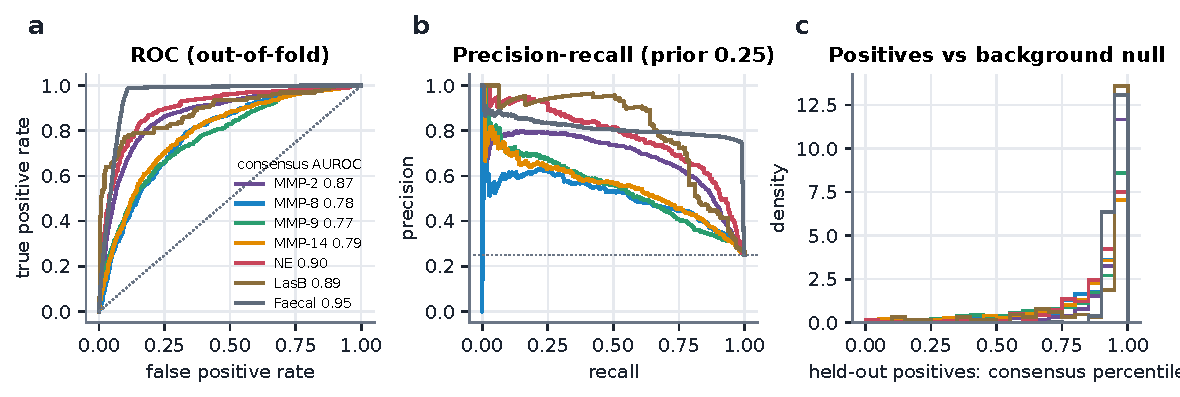
\includegraphics[width=\textwidth]{../figures/F09_roc_pr.pdf}
  \caption{Out-of-fold performance of the consensus score. \textbf{A:} ROC
    curves. \textbf{B:} precision-recall curves. \textbf{C:} distribution of the
    consensus percentile of held-out positives, which concentrates near the top
    of the background distribution for every protease.}
  \label{fig:roc}
\end{figure}

\subsection{Results: model and representation comparison}

Seven models were compared on identical folds: a constant prior, a
composition-only logistic regression, one-hot and VHSE logistic regressions, the
PSSM, and gradient-boosted trees on both encodings. Three conclusions follow.

\begin{itemize}[leftmargin=*,noitemsep]
\item \textbf{Position matters and composition mostly does not.} For six of
  seven proteases composition alone gives $0.60$--$0.74$ AUROC and the VHSE
  model exceeds it significantly; label-shuffled controls give
  \shuffleMin--\shuffleMax{}. LasB is the exception: composition alone reaches
  $0.886$, statistically indistinguishable from the full model. The LasB model
  therefore detects largely elastin-like composition, as expected from a
  positive set that is $76\%$ elastin \CONF.
\item \textbf{No strong position--position interaction is evident.}
  Gradient-boosted trees reach within $0.013$ AUROC of the better of the one-hot
  regression and the PSSM on every protease and exceed it only on NE, by $0.007$
  \CONF.
\item \textbf{The representation trade-off is real.} On data-rich proteases
  (MMP-2, MMP-8) the one-hot regression and the PSSM exceed the VHSE model
  significantly, by $0.017$ to $0.034$ AUROC, consistent with the bias measured
  by the subspace coverage below. On NE and LasB the VHSE model exceeds the
  one-hot regression significantly ($+0.021$ and $+0.033$). The learning curves
  show the same crossover: VHSE leads at small training sizes and is overtaken
  as data grow \CONF.
\end{itemize}

The PSSM has no fitted hyperparameter and lies at or within the interval of the
best model for every protease, which is the reason the shipped score combines it
with the logistic regression.

\begin{center}
\small\renewcommand{\arraystretch}{1.25}
\begin{tabular}{@{}lccccccc@{}}\toprule
Protease & Prior & Composition & One-hot LR & VHSE LR & PSSM & One-hot GBM & VHSE GBM \\\midrule
MMP-2 & 0.500 & 0.664 & 0.871 & 0.854 & \textbf{0.874} & 0.869 & 0.872 \\
MMP-8 & 0.500 & 0.596 & 0.777 & 0.750 & \textbf{0.784} & 0.780 & 0.783 \\
MMP-9 & 0.500 & 0.639 & 0.756 & 0.754 & \textbf{0.761} & 0.752 & 0.755 \\
MMP-14 & 0.500 & 0.633 & 0.772 & 0.771 & \textbf{0.785} & 0.773 & 0.779 \\
Neutrophil elastase & 0.500 & 0.676 & 0.866 & 0.887 & 0.885 & 0.892 & \textbf{0.894} \\
LasB & 0.500 & 0.886 & 0.845 & 0.877 & 0.881 & 0.878 & \textbf{0.889} \\
Faecal serine proteases & 0.500 & 0.742 & 0.952 & 0.951 & \textbf{0.953} & 0.950 & 0.951 \\
\bottomrule\end{tabular}

\end{center}

The table gives cross-validated AUROC by model (bold: best); the prior gives
$0.5$. The next table gives the AUROC of each alternative minus that of the VHSE
logistic regression under a paired cluster bootstrap (asterisk: $95\%$ interval
excludes zero).

\begin{center}
\small\renewcommand{\arraystretch}{1.25}
\begin{tabular}{@{}lcccc@{}}\toprule
Protease & One-hot LR & PSSM & One-hot GBM & VHSE GBM \\\midrule
MMP-2 & +0.017$^{*}$ & +0.020$^{*}$ & +0.015$^{*}$ & +0.018$^{*}$ \\
MMP-8 & +0.027$^{*}$ & +0.034$^{*}$ & +0.029$^{*}$ & +0.034$^{*}$ \\
MMP-9 & +0.003 & +0.008 & -0.002 & +0.001 \\
MMP-14 & +0.000 & +0.014$^{*}$ & +0.002 & +0.009 \\
Neutrophil elastase & -0.021$^{*}$ & -0.002 & +0.005 & +0.007 \\
LasB & -0.033$^{*}$ & +0.003 & +0.000 & +0.011 \\
Faecal serine proteases & +0.000 & +0.001 & -0.001 & -0.000 \\
\bottomrule\end{tabular}

\end{center}

\begin{figure}[H]
  \centering
  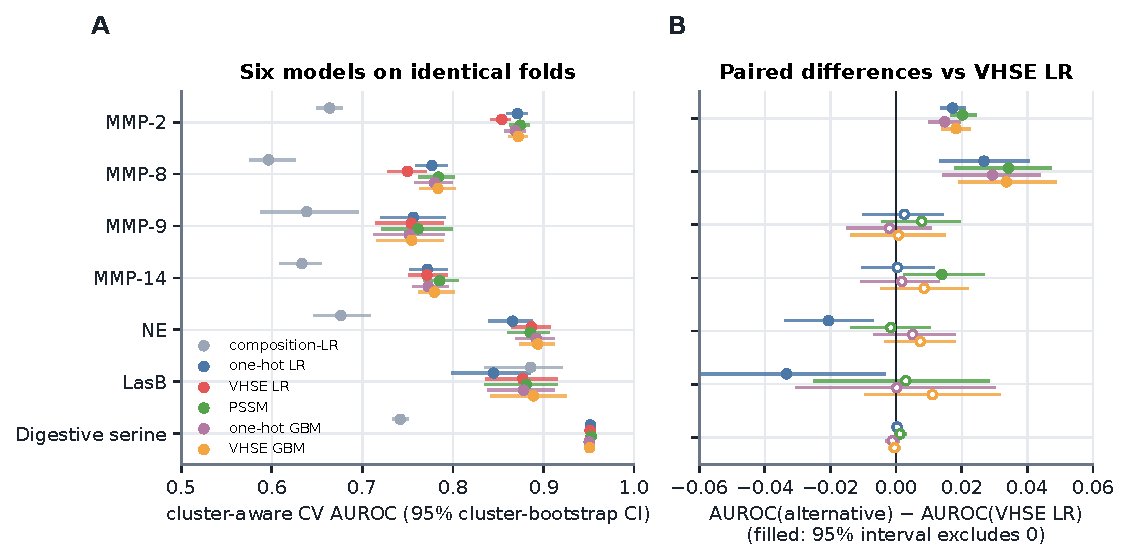
\includegraphics[width=\textwidth]{../figures/F05_model_comparison.pdf}
  \caption{\textbf{A:} cluster-aware AUROC of six models on identical folds with
    $95\%$ cluster-bootstrap intervals. \textbf{B:} paired difference
    (alternative minus VHSE logistic regression); filled markers have intervals
    excluding zero. The composition-only model lies $0.12$--$0.21$ below for every
    protease except LasB and is omitted from panel B for scale.}
  \label{fig:models}
\end{figure}

\begin{figure}[H]
  \centering
  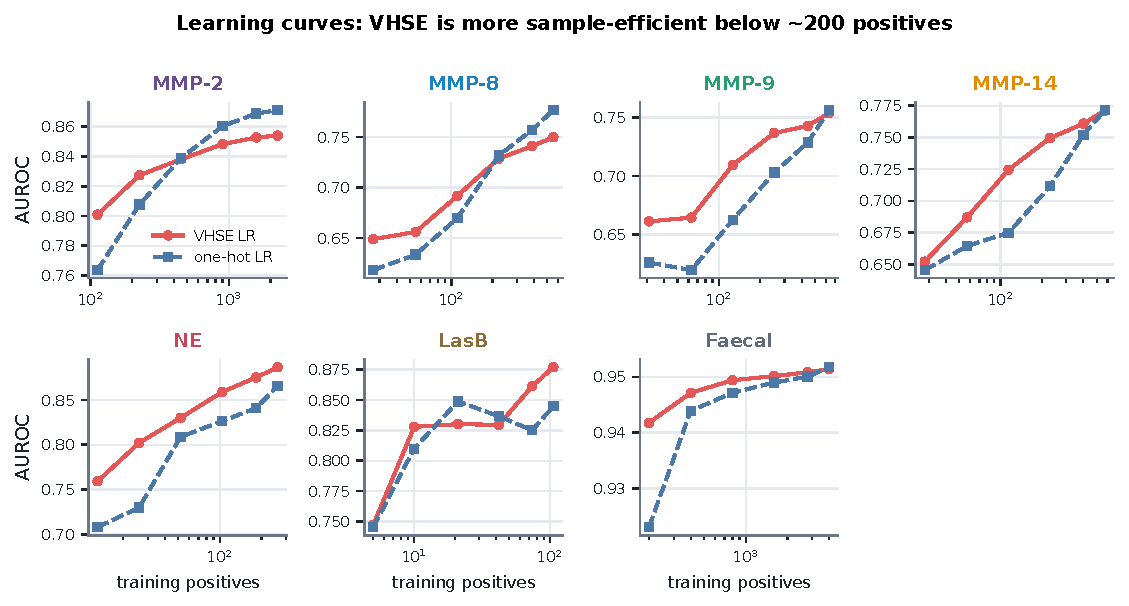
\includegraphics[width=\textwidth]{../figures/F06_learning_curves.pdf}
  \caption{Learning curves: AUROC as a function of the number of training
    positives for the VHSE and one-hot logistic regressions.}
  \label{fig:lc}
\end{figure}

\subsection{Results: training against other proteases}

Three negative-set designs were compared on a common held-out test set within
identical folds: composition-shuffled positives plus background (the earlier
design), background only, and the panel design of Part~\ref{sec:data}. Each was
scored on held-out target positives against background windows and against
held-out positives of the other proteases. The panel design costs
$0.01$--$0.02$ AUROC against background and gains against competitors on every
protease, most where it matters: for LasB from $0.80$ (background only) and
$0.68$ (shuffled) to $0.86$, for MMP-14 from $0.65$ to $0.73$, and for MMP-2
from $0.76$ to $0.79$ \CONF.

\begin{center}
\small\renewcommand{\arraystretch}{1.25}
\begin{tabular}{@{}lcccccc@{}}\toprule
 & \multicolumn{2}{c}{Shuffled + background} & \multicolumn{2}{c}{Background only} & \multicolumn{2}{c}{Panel (ours)} \\
\cmidrule(lr){2-3}\cmidrule(lr){4-5}\cmidrule(lr){6-7}
Protease & vs bkg & vs comp. & vs bkg & vs comp. & vs bkg & vs comp. \\\midrule
MMP-2 & 0.881 & 0.756 & 0.885 & 0.762 & 0.882 & 0.787 \\
MMP-8 & 0.834 & 0.654 & 0.828 & 0.651 & 0.810 & 0.683 \\
MMP-9 & 0.819 & 0.660 & 0.832 & 0.667 & 0.816 & 0.683 \\
MMP-14 & 0.831 & 0.660 & 0.833 & 0.649 & 0.811 & 0.727 \\
Neutrophil elastase & 0.850 & 0.910 & 0.852 & 0.900 & 0.848 & 0.926 \\
LasB & 0.801 & 0.676 & 0.889 & 0.798 & 0.891 & 0.863 \\
Faecal serine proteases & 0.954 & 0.939 & 0.954 & 0.938 & 0.953 & 0.944 \\
\bottomrule\end{tabular}

\end{center}

\begin{figure}[H]
  \centering
  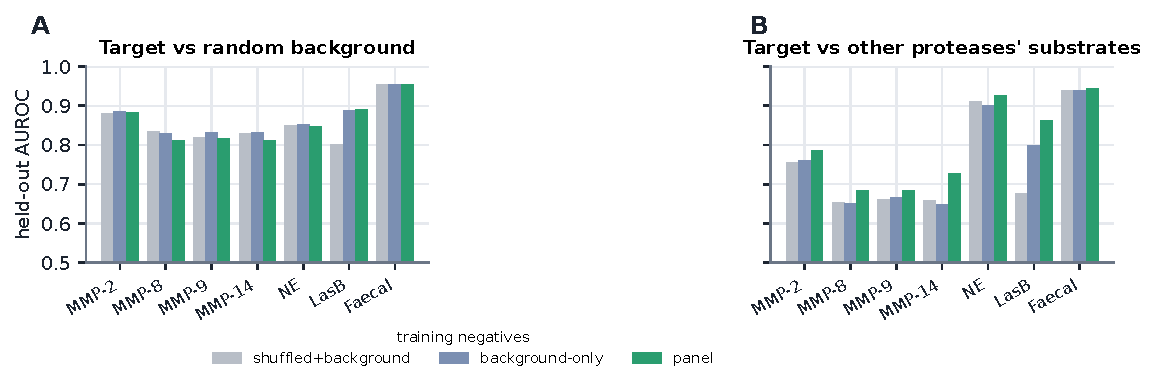
\includegraphics[width=\textwidth]{../figures/F07_negative_design.pdf}
  \caption{Effect of the training negatives on detection (\textbf{A}) and
    cross-protease discrimination (\textbf{B}).}
  \label{fig:neg}
\end{figure}

\subsection{Results: regularisation, leakage and controls}

Choosing $C$ by inner cross-validation raises or matches the $C=1$ default,
selecting $C=0.01$--$0.1$ for every protease except the faecal group. Random and
cluster-aware folds differ by at most \maxLeakGap{} AUROC, so near-duplicate
leakage is not a material source of optimism in these data, although the folds
guard against it. The table gives regularisation (AUROC at $C=1$ against nested
selection), fold construction (random against clustered, fixed $C=0.1$), the
label-shuffle control (mean of five permutations), and the variance-weighted
share of the learned PSSM log-odds that lies inside the VHSE subspace.

\begin{center}
\small\renewcommand{\arraystretch}{1.25}
\begin{tabular}{@{}lcccccc@{}}\toprule
 & \multicolumn{2}{c}{Regularisation} & \multicolumn{2}{c}{Fold construction} & Label & VHSE span \\
\cmidrule(lr){2-3}\cmidrule(lr){4-5}
Protease & $C=1$ & nested & random & clustered & shuffle & coverage \\\midrule
MMP-2 & 0.854 & 0.854 & 0.855 & 0.854 & 0.505 & 79\% \\
MMP-8 & 0.750 & 0.755 & 0.752 & 0.752 & 0.493 & 64\% \\
MMP-9 & 0.754 & 0.760 & 0.755 & 0.756 & 0.493 & 64\% \\
MMP-14 & 0.771 & 0.772 & 0.771 & 0.773 & 0.509 & 79\% \\
Neutrophil elastase & 0.887 & 0.895 & 0.897 & 0.895 & 0.495 & 65\% \\
LasB & 0.877 & 0.877 & 0.886 & 0.879 & 0.526 & 65\% \\
Faecal serine proteases & 0.951 & 0.951 & 0.951 & 0.951 & 0.494 & 77\% \\
\bottomrule\end{tabular}

\end{center}

\begin{figure}[H]
  \centering
  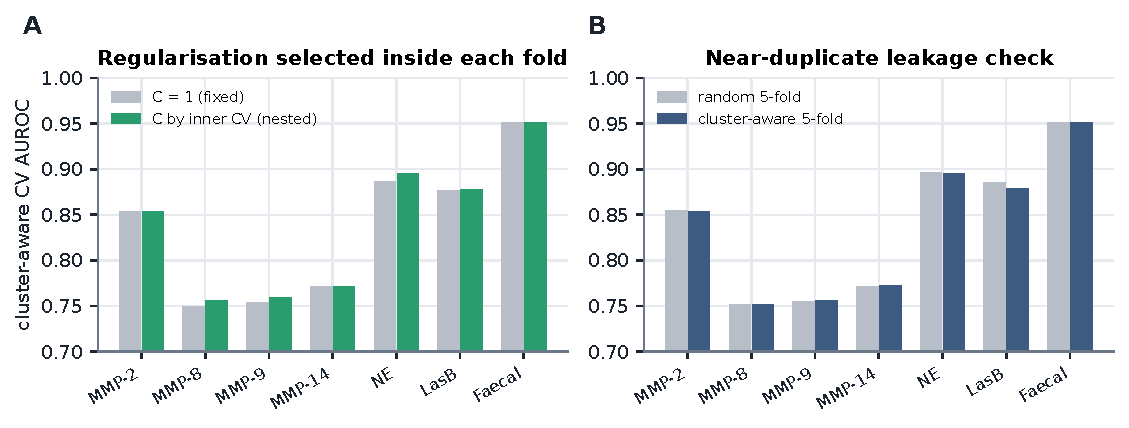
\includegraphics[width=\textwidth]{../figures/F08_tuning_and_leakage.pdf}
  \caption{\textbf{A:} nested regularisation selection against fixed $C=1$.
    \textbf{B:} random against cluster-aware folds.}
  \label{fig:tune}
\end{figure}

\subsection{Results: calibration and scale}

Reliability curves of the logistic-regression score lie below the diagonal:
with balanced class weights the score is a posterior under a $50{:}50$ prior,
whereas the training mixture has a positive prior of $0.25$ and real sequences a
far lower one. Expected calibration error is $0.06$--$0.20$. Base rates also
differ by model, the mean score on random windows ranging from $0.11$ (faecal
group) to $0.35$ (MMP-14), which motivates the percentile scale of
Part~\ref{sec:panel} \CONF.

\begin{figure}[H]
  \centering
  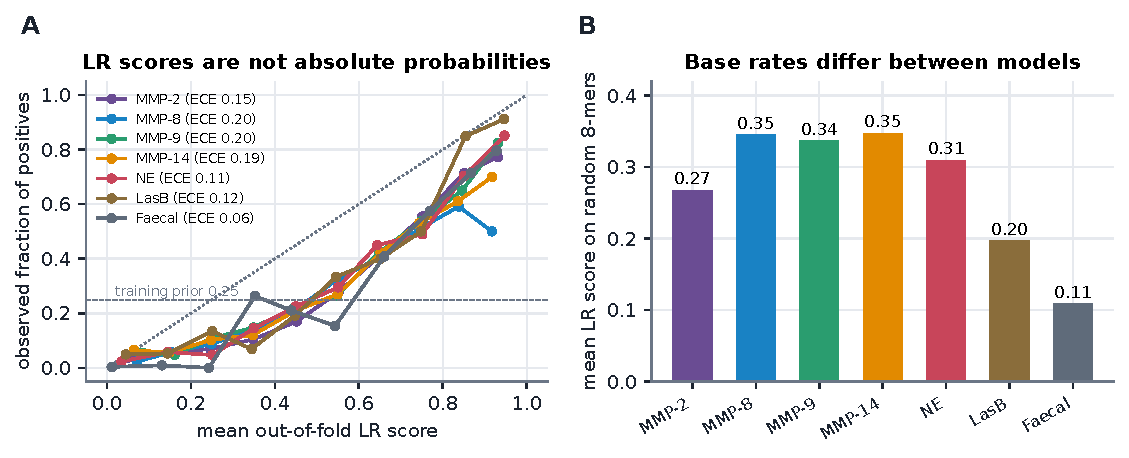
\includegraphics[width=\textwidth]{../figures/F10_calibration.pdf}
  \caption{\textbf{A:} reliability curves of the out-of-fold
    logistic-regression score. \textbf{B:} mean logistic-regression score on
    random background windows for each final model.}
  \label{fig:calib}
\end{figure}

\subsection{Results: selectivity between proteases}

The next table gives, for each target model, the held-out AUROC for separating
the target's substrates from a competitor's substrates (the competitor's windows
were training negatives, but each is scored out-of-fold). The NE and faecal
models separate their substrates from every competitor's at $0.90$--$0.98$. The
MMP models separate theirs from NE's at $0.89$--$0.93$, but from LasB's and the
faecal group's at only $0.63$--$0.89$. Within the MMP family discrimination is
modest ($0.53$--$0.72$), lowest for MMP-14 against MMP-2 ($0.53$) and MMP-8 against
MMP-2 ($0.57$) \CONF.

\begin{center}
\small\renewcommand{\arraystretch}{1.25}
\begin{tabular}{@{}lccccccc@{}}\toprule
Target model & MMP-2 & MMP-8 & MMP-9 & MMP-14 & NE & LasB & Faecal \\\midrule
MMP-2 & -- & 0.72 & 0.68 & 0.69 & 0.93 & 0.79 & 0.89 \\
MMP-8 & 0.57 & -- & 0.58 & 0.64 & 0.91 & 0.82 & 0.63 \\
MMP-9 & 0.59 & 0.65 & -- & 0.70 & 0.90 & 0.63 & 0.63 \\
MMP-14 & 0.53 & 0.62 & 0.70 & -- & 0.89 & 0.80 & 0.84 \\
Neutrophil elastase & 0.93 & 0.93 & 0.93 & 0.94 & -- & 0.92 & 0.96 \\
LasB & 0.84 & 0.90 & 0.81 & 0.84 & 0.87 & -- & 0.91 \\
Faecal & 0.96 & 0.90 & 0.91 & 0.96 & 0.98 & 0.97 & -- \\
\bottomrule\end{tabular}

\end{center}

\begin{figure}[H]
  \centering
  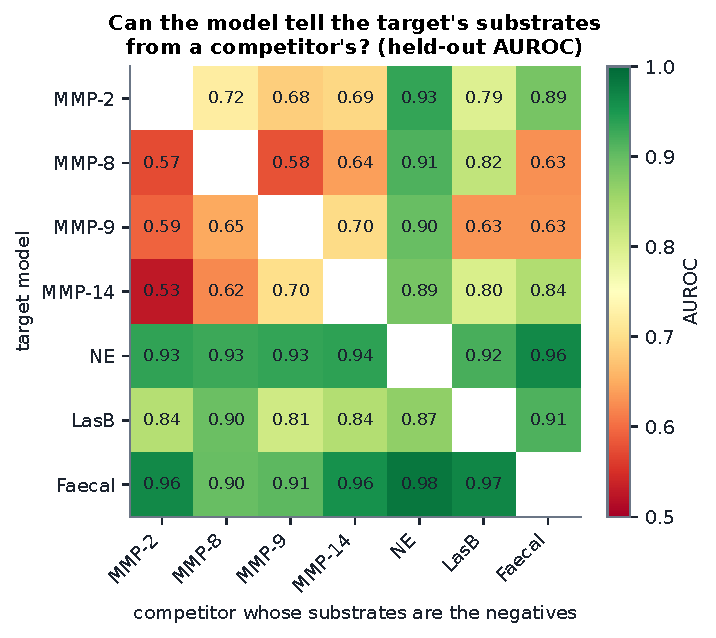
\includegraphics[width=0.62\textwidth]{../figures/F11_selectivity_matrix.pdf}
  \caption{Cross-protease discrimination matrix (data of the preceding table).}
  \label{fig:selmat}
\end{figure}

A low competitor AUROC does not by itself indicate a poor model. By
Eq.~\eqref{eq:contam}, if a fraction $\pi$ of a competitor's substrates are also
cleaved by the target, the measured AUROC is at most $1-\pi/2$ for a perfect
model. Exact-window overlap between protease positive sets is small, but the MMPs
share their dominant preferences \cit{1}, so many competitor windows are
plausibly cleaved by the target as well; the ceiling for MMP-against-MMP AUROC is
therefore below $1$ by an amount that sequence data alone cannot measure
\FLAG. The practical conclusion is unchanged: from a P4--P4$'$ window alone the
MMPs cannot be reliably distinguished, and a sensor design should not depend on
it.

\begin{figure}[H]
  \centering
  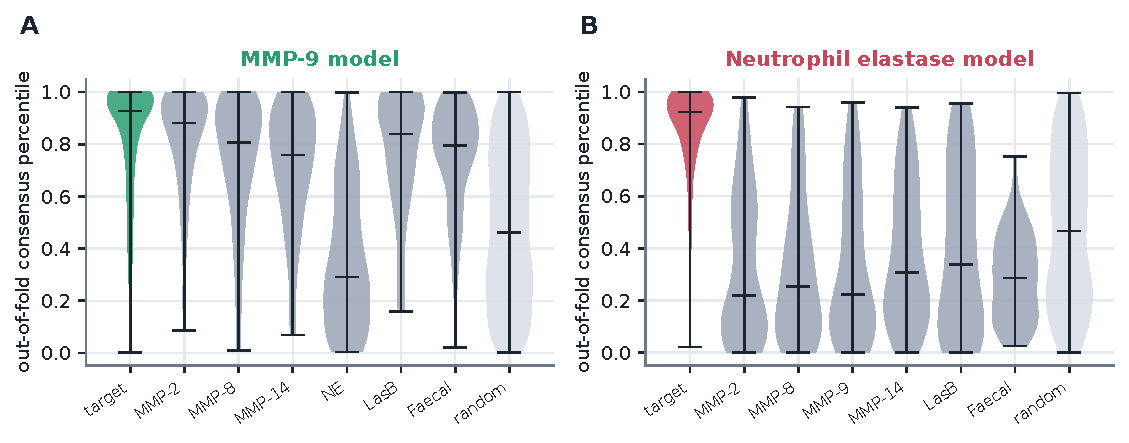
\includegraphics[width=\textwidth]{../figures/F16_score_distributions.pdf}
  \caption{Out-of-fold consensus percentiles of held-out positives (target) and
    of each competitor's substrates and random windows for the MMP-9 model
    (\textbf{A}) and the NE model (\textbf{B}). The MMP-9 model places MMP-2 and
    MMP-8 substrates almost as high as its own; the NE model separates them
    sharply.}
  \label{fig:dist}
\end{figure}

\subsection{Results: what the models learned}

Coefficient stability by cluster bootstrap identifies which learned effects are
reliable: between $17$ (MMP-14) and $35$ (MMP-2) of the $64$ standardised
coefficients per model have $95\%$ intervals excluding zero, so the
position-level pattern is more trustworthy than any single descriptor weight.
Total contribution is concentrated at $\pos{3}$ and $\prm{1}$ for the MMPs, at
$\pos{1}$ for NE and the faecal group, and is spread across positions for LasB;
the electronic family, which accounts for four of the eight descriptors, carries
the largest share for every protease.

\begin{figure}[H]
  \centering
  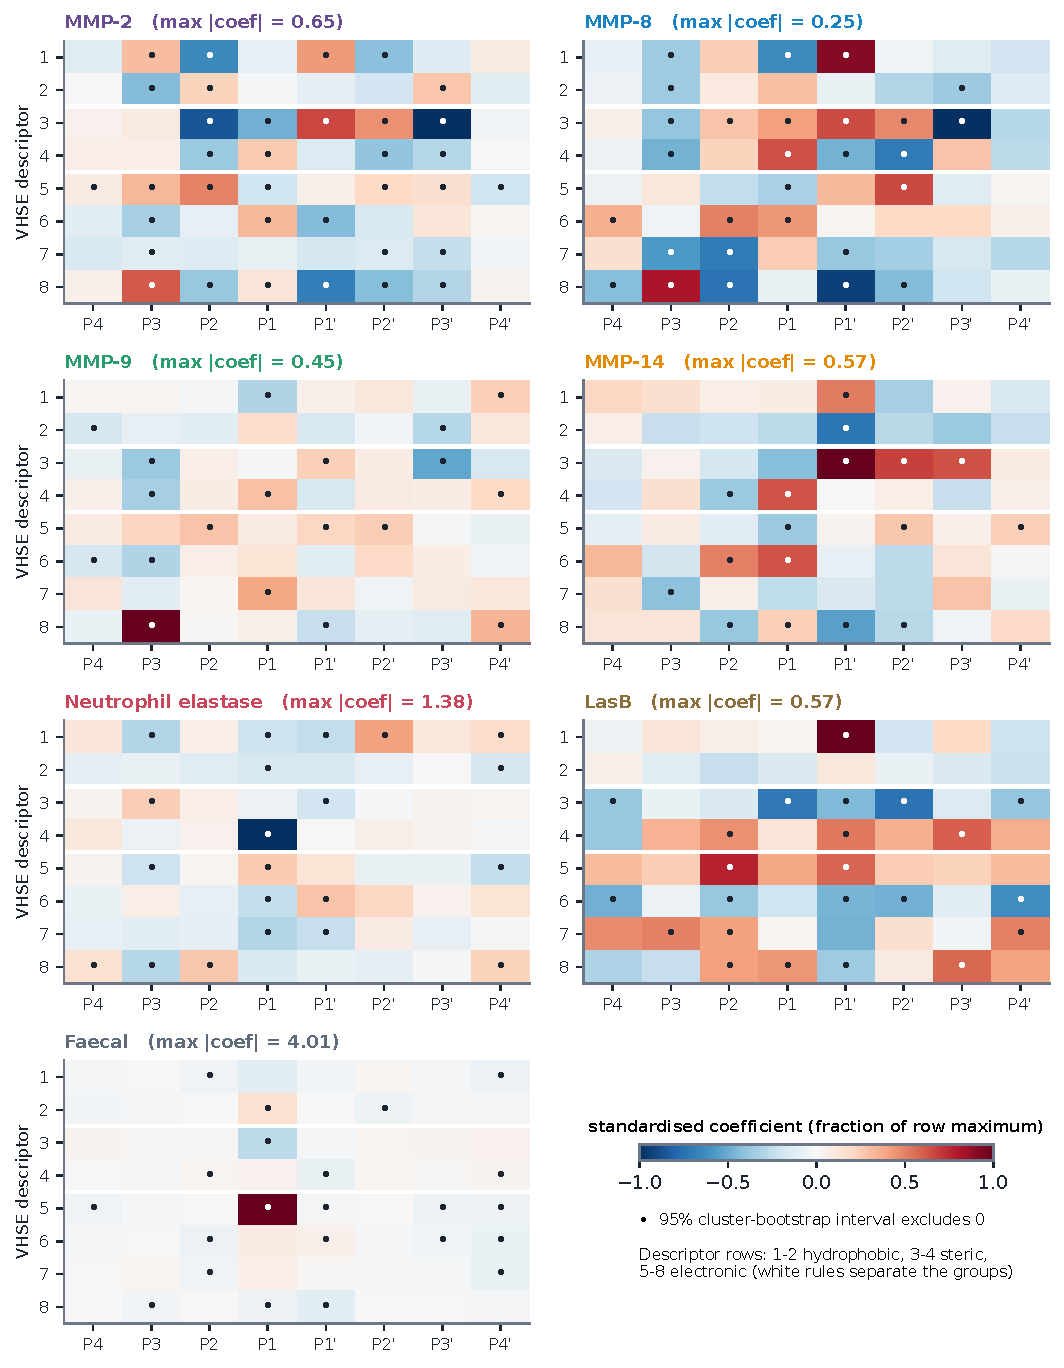
\includegraphics[width=0.97\textwidth]{../figures/F12_coefficients.pdf}
  \caption{Standardised logistic-regression coefficients by position and VHSE
    descriptor. Dots mark coefficients whose $95\%$ cluster-bootstrap interval
    excludes zero. Colours are scaled to each protease's largest coefficient.}
  \label{fig:coef}
\end{figure}

\begin{figure}[H]
  \centering
  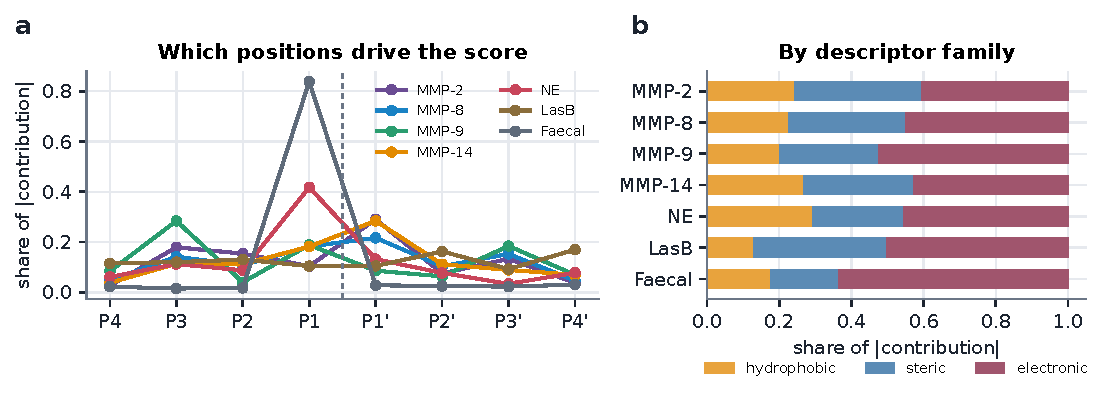
\includegraphics[width=\textwidth]{../figures/F13_position_importance.pdf}
  \caption{\textbf{A:} share of mean absolute logit contribution by position,
    computed on training positives. \textbf{B:} share by descriptor family.}
  \label{fig:pos}
\end{figure}

%=======================================================================
\section{Part E: Validation Against Published Data and Structures}
\label{sec:valid}

\subsection{Overview}

Cross-validation shows that the models generalise within their data-generating
process. Three comparisons that do not share that process are reported: whether
the model recovers published specificity that it was not shown, whether the
active-site structure of the enzymes agrees with what it learned, and whether
its scores rank measured kinetics.

\subsection{Assumptions}

\begin{assump}
\begin{itemize}[leftmargin=*,noitemsep]
\item \textbf{The phage-display consensus of Kridel et al.\ is independent of
  the training data.} It derives from a different experiment and is not in
  MEROPS or PICS \cit{1} \FLAG.
\item \textbf{Kinetic values are transcribed from Table~II of the source.} All
  twelve rows were extracted programmatically and checked against the paper
  \cit{1} \CONF.
\item \textbf{Peptides shorter than eight positions around the bond are scored
  as gapped windows.} The peptides are N-acetylated and C-amidated, so
  $\prm{4}$ is absent for most of them \CONF.
\item \textbf{The validation set is small and pre-selected.} Eleven peptides,
  all selected for MMP-9 activity, with no MMP-13 or MMP-7 model available to
  test the reported selectivity \CONF.
\end{itemize}
\end{assump}

\subsection{Recovery of the MMP-9 consensus}

The consensus of Kridel et al., Pro-Arg-Ser/Thr$\downarrow$Hy-Ser/Thr, is
overlaid on the learned MMP-9 PSSM below. Pro at $\pos{3}$ is the top-ranked
residue of twenty ($\pssmLOPThreePro$ bits), Leu and Ile are first and second
at $\prm{1}$ ($\pssmLOPOnePLeu$ and $\pssmLOPOnePIle$ bits), and Arg at $\pos{2}$
ranks \pssmRankPTwoArg{} of $20$ ($\pssmLOPTwoArg$ bits) \CONF. These are the two
features that Kridel et al.\ associate with specific enzyme pockets: an S3
subsite that accommodates the bend introduced by Pro, and the deep hydrophobic
S1$'$ pocket.

Ser/Thr at $\pos{1}$ and $\prm{2}$ is not reproduced (Thr ranks
\pssmRankPOneThr{} of $20$ at $\pos{1}$, $\pssmLOPOneThr$ bits; Ser ranks
\pssmRankPTwoPSer{} at $\prm{2}$). This is consistent with the report of Kridel
et al.\ that about two thirds of the $\prm{2}$ Thr residues in the selected
clones are encoded by the phage vector rather than selected. At $\pos{1}$ the
top residues are Gly, Lys and Arg ($\pssmLOPOneGly$, $\pssmLOPOneLys$,
$\pssmLOPOneArg$ bits); Gly at $\pos{1}$ is the pattern of the natural collagen
substrates in Table~III of the same source, and Arg at $\pos{1}$ is favoured in
their group~III substrates. The learned specificity is that of natural and
proteome-derived sites, which differs from a phage-optimised consensus at the
positions where that difference is expected.

\begin{figure}[H]
  \centering
  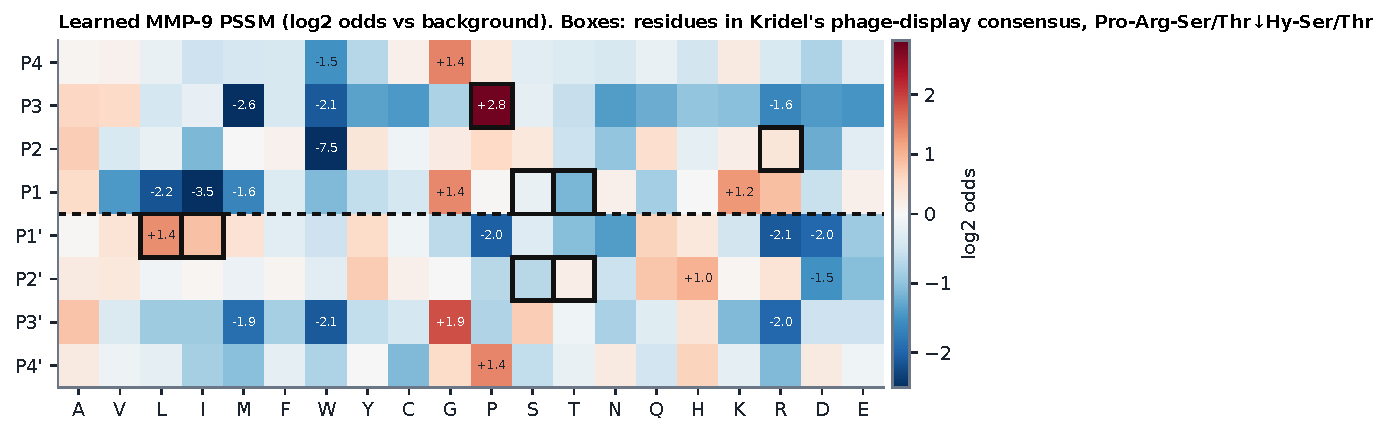
\includegraphics[width=\textwidth]{../figures/F14_mmp9_consensus.pdf}
  \caption{Learned MMP-9 PSSM (log$_2$ odds against background; cells with
    $|{\cdot}|>1$ bit are annotated). Boxes mark the residues of the Kridel et al.\
    phage-display consensus. Pro at $\pos{3}$ and Leu/Ile at $\prm{1}$ are
    recovered; Ser/Thr at $\pos{1}$ and $\prm{2}$ are not.}
  \label{fig:kcons}
\end{figure}

\subsection{Learned specificity and the enzyme structures}
\label{sec:structures}

One experimental structure per protease was prepared (table below), and
active-site facts were derived from the coordinates. In MMP-9, MMP-2 and MMP-8
the sequence around the catalytic zinc reads H-E-F-G-H-A-L-G-L-D/E-H, the
HEXXHXXGXXH motif of Nagase and Woessner \cit{2} \CONF; the zinc is coordinated
by the two histidines of HEXXH and the third histidine of the motif (His401,
His405 and His411 in MMP-9), and the hydroxamate oxygen of the bound MMP-9
inhibitor lies $2.07$~\AA\ from it \CONF. In LasB the zinc ligands are His140,
His144 and Glu164; in neutrophil elastase the catalytic triad is His57, Asp102
and Ser195 \CONF. Residues lining the ligand-occupied pocket of MMP-9 include
Asp185-Gly186-Leu187, the Asp-Gly-Leu segment that Kridel et al.\ assign to the
S2$'$ subsite (their numbering differs), and Met422. In NE they include Val190,
Ala213 and Val216, small aliphatic side chains, and the top residues of the NE
model at $\pos{1}$ are Val, Ile and Thr.

\begin{center}
\small\renewcommand{\arraystretch}{1.25}
\begin{tabular}{@{}llcclc@{}}\toprule
Protease & PDB & Resolution (\AA) & Residues & Catalytic site residues & Pocket residues \\\midrule
MMP-2 & 1QIB & 2.8 & 160 & HIS201, HIS205, HIS211 & 23 \\
MMP-8 & 1JAN & 2.5 & 164 & HIS197, HIS201, HIS207 & 21 \\
MMP-9 & 1GKC & 2.3 & 159 & HIS401, HIS405, HIS411 & 20 \\
Neutrophil elastase & 1HNE & 1.84 & 210 & ASP102, HIS57, SER195 & 22 \\
LasB & 1EZM & 1.5 & 298 & GLU164, HIS140, HIS144 & 27 \\
\bottomrule\end{tabular}

\end{center}

The table lists the structures used. Catalytic-site residues are those
coordinating the catalytic zinc (MMPs, LasB) or forming the catalytic triad
(NE); pocket residues lie within $6$~\AA\ of the bound ligand, or within
$9$~\AA\ of the catalytic zinc when no ligand is present. MMP-9 is taken from an
active catalytic-domain entry rather than the pro-form, whose prodomain occupies
the cleft \cit{10}.

\begin{figure}[H]
  \centering
  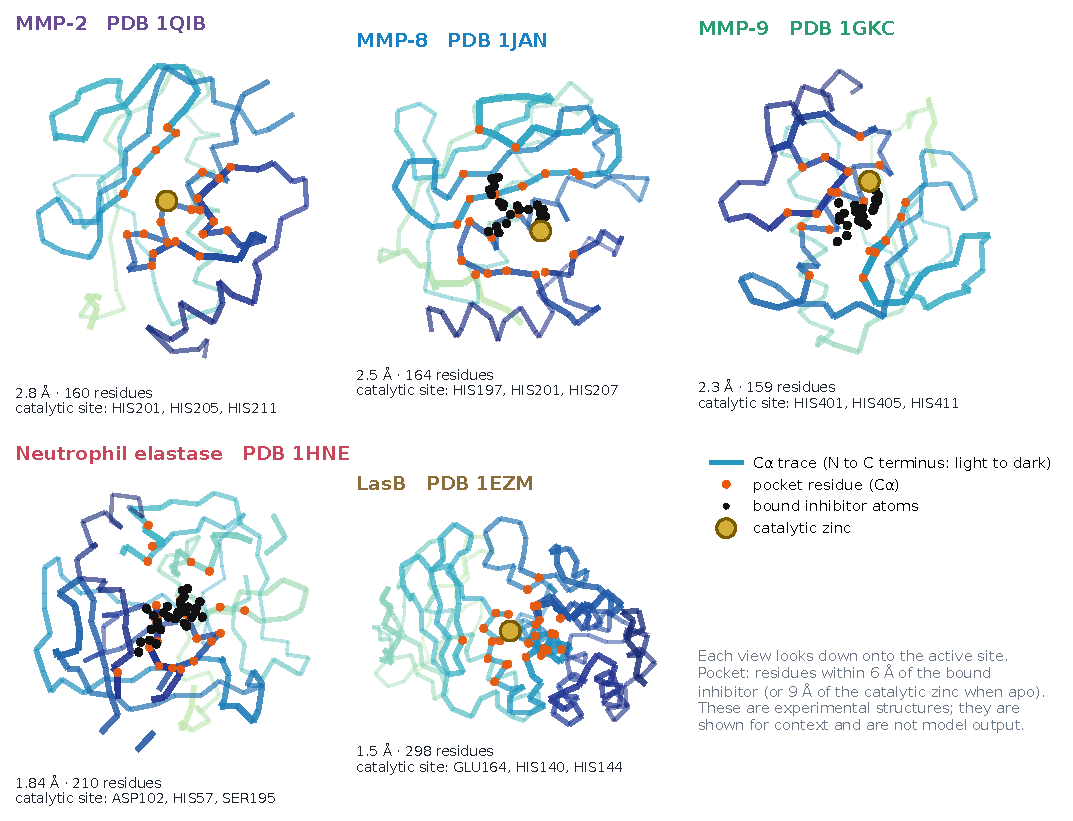
\includegraphics[width=\textwidth]{../figures/F19_structures.pdf}
  \caption{C$\alpha$ traces of the five structures, each oriented toward the
    active site (depth-cued; N to C terminus from light to dark). Orange: pocket
    residues; gold: catalytic zinc; black: bound inhibitor atoms. The structures
    are experimental and are shown for context; they are not model output.}
  \label{fig:struct}
\end{figure}

\subsection{Held-out measured kinetics}

Kridel et al.\ \cit{1} measured $\kcat/\Km$ for MMP-9 on eleven synthetic
peptides and detected no activity on a twelfth (C11). Training windows that
coincide with a validation peptide on at least seven positions (four windows)
were removed from every training set and the MMP-9 model was retrained before
scoring. Each peptide was scored as a gapped window and rank-correlated with
$\log_{10}\kcat/\Km$.

\begin{center}
\small\renewcommand{\arraystretch}{1.25}
\begin{tabular}{@{}llrrrr@{}}\toprule
Peptide & Window (P4--P4$'$) & Positions & MMP-9 $k_\mathrm{cat}/K_m$ (M$^{-1}$s$^{-1}$) & LR logit & PSSM \\\midrule
C15 & \texttt{GPRQITA-} & 7 & 188{,}000 & +2.07 & +5.41 \\
A11 & \texttt{IPRTLTA-} & 7 & 67{,}500 & +1.30 & +3.67 \\
A6 & \texttt{GPRAVSTT} & 8 & 61{,}000 & +1.24 & +4.20 \\
A11m1 & \texttt{IPRRLTA-} & 7 & 160{,}000 & +2.43 & +5.66 \\
A11m2 & \texttt{IPRTATA-} & 7 & 2{,}000 & +1.15 & +2.35 \\
A10 & \texttt{GPLFYSVT} & 8 & 25{,}600 & +0.33 & +2.70 \\
B1 & \texttt{QPHYLTTA} & 8 & 8{,}800 & +0.81 & +3.10 \\
A18 & \texttt{RPAKSTA-} & 7 & 5{,}800 & +1.28 & +4.96 \\
A7 & \texttt{--SGLKAL} & 6 & 12{,}400 & +0.77 & +3.08 \\
A19 & \texttt{GSRYLTA-} & 7 & 13{,}200 & +0.74 & +3.02 \\
A16 & \texttt{SGRRLLSR} & 8 & 1{,}200 & +0.68 & +0.78 \\
C11 & \texttt{SGRRLIHH} & 8 & not detected & +0.30 & +2.47 \\
\bottomrule\end{tabular}

\end{center}

The table lists the validation peptides as P4--P4$'$ windows with measured
$\kcat/\Km$ and the scores of the retrained model. The next table gives the
rank association; the permutation $p$-value is two-sided, intervals are
bootstrap intervals over peptides, and the last rows rank C11 below every
measured peptide.

\begin{center}
\small\renewcommand{\arraystretch}{1.25}
\begin{tabular}{@{}llccc@{}}\toprule
Score & Set & Spearman $\rho$ & 95\% bootstrap CI & Permutation $p$ \\\midrule
Logistic regression & n = 11 measured & 0.58 & [-0.23, 0.93] & 0.068 \\
Logistic regression & n = 12 (C11 ranked lowest) & 0.68 & [0.02, 0.96] & 0.017 \\
PSSM & n = 11 measured & 0.70 & [-0.00, 0.96] & 0.020 \\
PSSM & n = 12 (C11 ranked lowest) & 0.75 & [0.18, 0.93] & 0.006 \\
Standardised mean & n = 11 measured & 0.57 & [-0.21, 0.90] & 0.074 \\
Standardised mean & n = 12 (C11 ranked lowest) & 0.66 & [0.06, 0.91] & 0.021 \\
\bottomrule\end{tabular}

\end{center}

The association is positive for every scorer and set. For the PSSM,
$\rho=\rhoNElevenPSSM$ on the eleven measured peptides (permutation
$p=\rhoPNElevenPSSM$; $95\%$ interval $[\rhoLoNElevenPSSM,\rhoHiNElevenPSSM]$);
for the logistic regression $\rho=\rhoNElevenLR$ ($p=\rhoPNElevenLR$). The
intervals are wide and, for the logistic regression on $n=11$, include zero.
With $n=11$ and a set that was itself selected for high activity, this is
evidence of a positive association and not of accurate rate prediction, and the
six tests are not corrected for multiplicity. By the logistic regression the
three highest-scored peptides (A11m1, C15, A11) are the three most active; its
largest miss is A10 ($25{,}600$~M$^{-1}$s$^{-1}$, the fifth most active), which it
scores second-lowest. The PSSM scores the least active measured peptide (A16)
lowest but ranks A18 ($5{,}800$) third, its largest miss.

\begin{figure}[H]
  \centering
  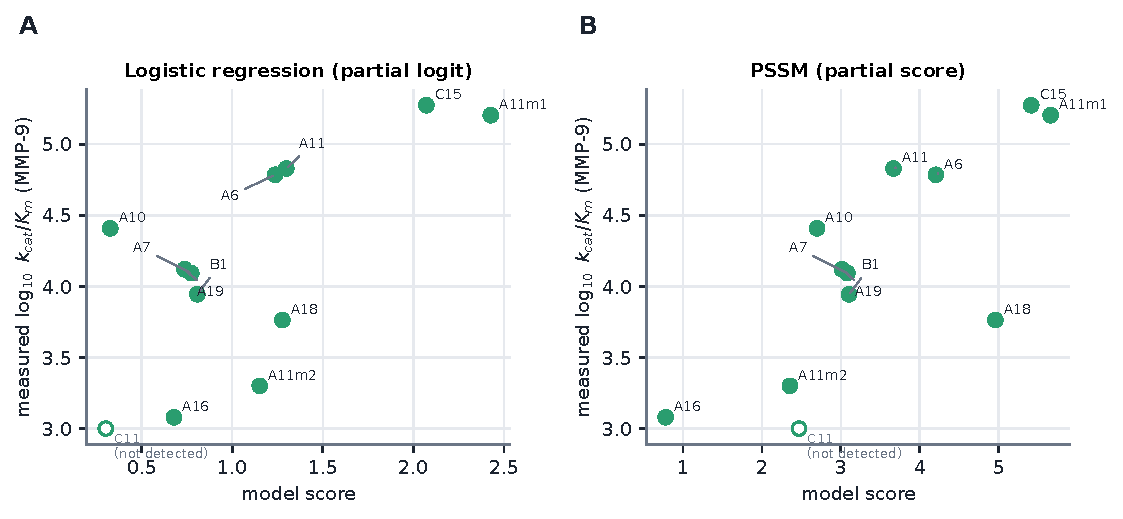
\includegraphics[width=\textwidth]{../figures/F15_kridel_validation.pdf}
  \caption{Model score against measured MMP-9 $\log_{10}\kcat/\Km$. Open marker:
    C11, no activity detected (plotted at the floor of the axis).}
  \label{fig:kval}
\end{figure}

\subsection{Matched point mutants}

Two peptides are single-substitution mutants of A11 (SGKIPRT$\downarrow$LTA):
A11m1 replaces Thr with Arg at $\pos{1}$; A11m2 replaces Leu with Ala at
$\prm{1}$. Because the background is identical, each isolates one substitution.

\begin{center}
\small\renewcommand{\arraystretch}{1.25}
\begin{tabular}{@{}llccc@{}}\toprule
Pair & Substitution & Measured fold change (log$_2$) & LR $\Delta$ (bits) & PSSM $\Delta$ (bits) \\\midrule
A11$\to$A11m1 & T7R at P1 (Thr to Arg) & 2.37$\times$ (+1.25) & +1.63 & +1.99 \\
A11$\to$A11m2 & L8A at P1' (Leu to Ala) & 0.03$\times$ (-5.08) & -0.21 & -1.31 \\
\bottomrule\end{tabular}

\end{center}

The model predicts the correct direction for both and approximately the correct
size for the first ($+\mutOneLR$ bits from the logistic regression and
$+\mutOnePSSM$ from the PSSM, against a measured $+\mutOneMeasured$ log$_2$
units). For the second it predicts a decrease but underestimates it:
$\mutTwoLR$ bits (logistic regression) and $\mutTwoPSSM$ bits (PSSM) against a
measured $\mutTwoMeasured$. Large kinetic effects of a single key residue are
compressed by a model trained to distinguish cleaved from uncleaved sites, not
fast from slow \CONF.

%=======================================================================
\section{Part F: Application to Sensor Candidate Design}
\label{sec:design}

\subsection{Overview}

The candidate design analysis defines sensor cores as short motifs and scores
them as eight-residue windows. Three of the four cores, PRSLSGLK, PLGLAGQS and
PLGVALAA, are motifs whose scissile bond lies after the third residue
(Pro-Arg-Ser$\downarrow$Leu and Pro-Leu-Gly$\downarrow$Leu, with $\pos{3}=\mathrm{Pro}$
and $\prm{1}=\mathrm{Leu}$, matching the consensus of Kridel et al.\ \cit{1}).
Read as a P4--P4$'$ window, whose bond follows the fourth character, every
residue is displaced by one position from its intended subsite: for PRSLSGLK the
window has $\pos{2}=\mathrm{S}$ and $\prm{1}=\mathrm{S}$ in place of
$\pos{2}=\mathrm{R}$ and $\prm{1}=\mathrm{L}$. The design plan itself states the
intended features as $\pos{2}=\mathrm{Arg}$, $\prm{1}=\mathrm{Leu}$,
$\prm{2}=\mathrm{Ser}$, which the displaced window does not encode.

\subsection{Assumptions}

\begin{assump}
\begin{itemize}[leftmargin=*,noitemsep]
\item \textbf{The scissile bond of each core lies where its motif places it.}
  After the third residue for the Pro-X-X$\downarrow$Leu cores and after the
  fourth for AAPV$\downarrow$SGIG \FLAG.
\item \textbf{Device constraints are those of the design filter.} No Cys
  (reserved for the gold-thiol anchor), no Trp (electroactive near the methylene
  blue window), net charge $-1$ to $+2$, no Pro-Pro, core mass $600$--$1100$~Da.
  These are team design rules, not model output \CONF.
\item \textbf{Optimised sequences extrapolate.} Candidates selected from a
  random pool lie far from any training window, where neither the models nor
  their percentile scales have been checked \FLAG.
\end{itemize}
\end{assump}

\subsection{Equations}

Each candidate carries the position after which its bond lies and is scored as a
gapped window (Part~\ref{sec:panel}): unknown positions (the $\pos{4}$ of the
three cores, and any residue beyond $\prm{4}$) are marginalised as described
there, and percentiles use a null with the same positions masked. The
specificity margin is Eq.~\eqref{eq:margin}.

\subsection{Results: effect of the alignment correction}

The model responded correctly to the displaced input: PRSLSGLK scored at the
$7$th percentile for MMP-9. Scored as the gapped window \texttt{-PRSLSGL} with
the bond after the third residue, it scores at the $100$th percentile, and at
the top for MMP-2 and MMP-8 as well. The correction also changes a design
conclusion. The $3\times3$ specificity matrix of the MMP-2/MMP-9/NE design
analysis has condition number $61.7$ with the displaced windows (poorly
conditioned; pivot to a two-plex, by the analysis's own rule) and $16.1$ with
the corrected windows (marginal). The corrected matrix still shows that the
MMP-2 and MMP-9 candidates are not separable by score, as the selectivity
results of Part~\ref{sec:eval} predict \CONF.

\begin{center}
\small\renewcommand{\arraystretch}{1.25}
\begin{tabular}{@{}llllcc@{}}\toprule
Candidate & Core & Scored window & Target & Margin (3-plex) & Pool percentile \\\midrule
Cand1 MMP9 & \texttt{PRSLSGLK} & \texttt{-PRSLSGL} & MMP-9 & -0.00 & 16 \\
Cand2 MMP2 & \texttt{PLGLAGQS} & \texttt{-PLGLAGQ} & MMP-2 & -0.00 & 0 \\
Cand4 NE & \texttt{AAPVSGIG} & \texttt{AAPVSGIG} & NE & +0.51 & 26 \\
Cand3 MMP2b & \texttt{PLGVALAA} & \texttt{-PLGVALA} & MMP-2 & -0.04 & 0 \\
\bottomrule\end{tabular}

\end{center}

The table gives the candidates scored in the MMP-2/MMP-9/NE panel with correctly
aligned, gapped windows; the pool percentile is that of the margin within the
PSSM top-3 enumeration pool for the target, with the same gap pattern.

\subsection{Results: candidate landscape in the wound panel}

The figure and table below rank candidates in the five-protease wound panel
(MMP-2, MMP-8, MMP-9, NE, LasB). The pool combines $150{,}000$ random windows with
the PSSM top-3 enumerations of each target, filtered by the device constraints.

\begin{itemize}[leftmargin=*,noitemsep]
\item \textbf{The best-scoring sequences are model optima, not
  recommendations.} They are extreme points of a search over a random pool and
  are hypotheses for wet-lab testing.
\item \textbf{The MMP-family reference cores have margin near zero.} The
  corrected MMP-9 cores (\texttt{IPRTLTA-} and \texttt{-PRSLSGL}) score at the top
  for MMP-2, MMP-8 and MMP-9 alike, so no selectivity among MMPs is predicted.
  Kridel et al.\ found A11 to be $2.9$-fold and $9.6$-fold more active on MMP-9
  than on MMP-13 and MMP-7 \cit{1}; neither is in the panel, so this cannot be
  tested here.
\item \textbf{The panel changes the answer.} AAPVSGIG has margin $+0.51$ in the
  three-protease panel and $0.00$ in the wound panel, because the LasB model,
  trained largely on Gly/Ala/Pro-rich elastin sequence, scores it at the $99$th
  percentile. Whether LasB cleaves AAPV-type sites cannot be settled from these
  data \FLAG.
\end{itemize}

\begin{figure}[H]
  \centering
  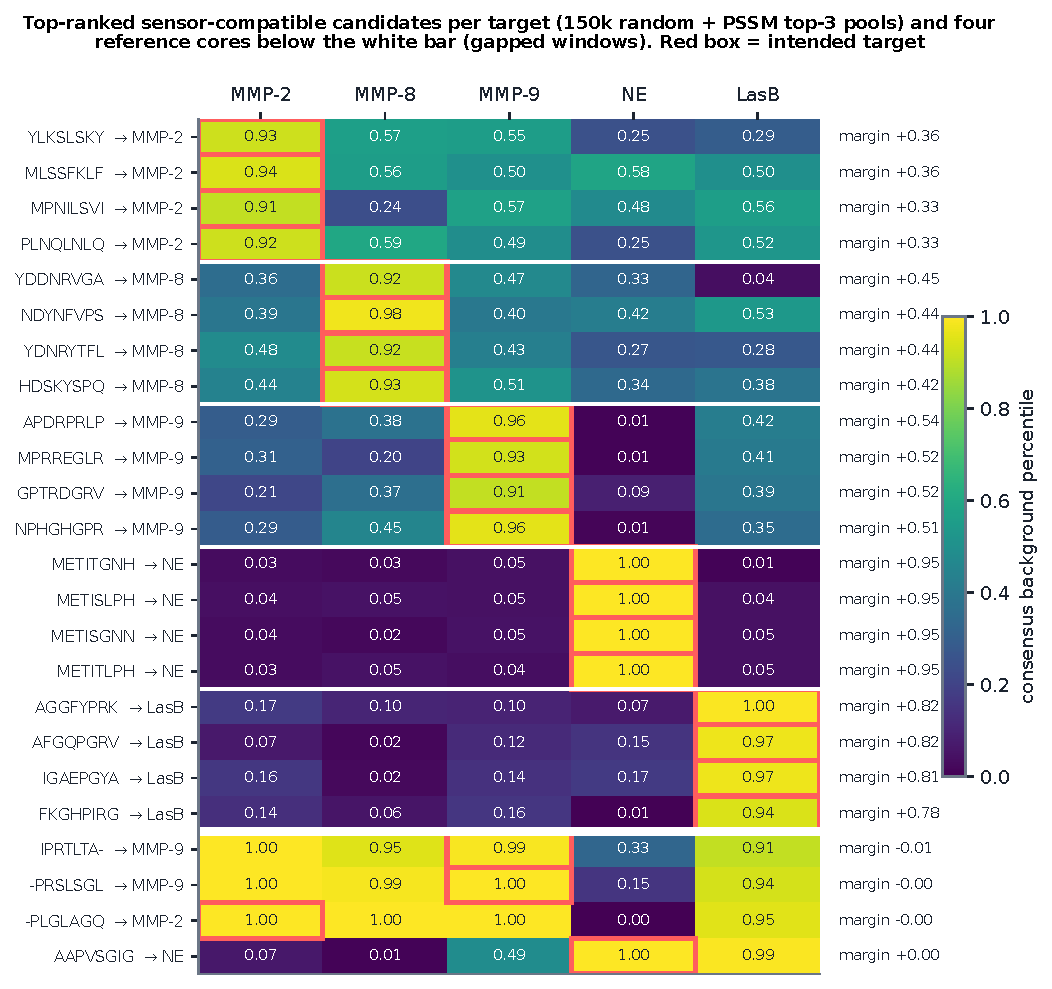
\includegraphics[width=0.85\textwidth]{../figures/F17_candidate_landscape.pdf}
  \caption{Consensus background percentiles of the four highest-margin
    sensor-compatible candidates for each target (above the white bar) and of
    four reference cores (below), across the five wound-panel proteases. Red
    boxes mark the intended target; margins are listed at the right. Reference
    cores are scored as gapped windows.}
  \label{fig:cand}
\end{figure}

\begin{center}
\small\renewcommand{\arraystretch}{1.25}
\begin{tabular}{@{}llccccc c@{}}\toprule
Window & Target & MMP-2 & MMP-8 & MMP-9 & NE & LasB & Margin \\\midrule
\texttt{YLKSLSKY} & MMP-2 & 0.93 & 0.57 & 0.55 & 0.25 & 0.29 & +0.36 \\
\texttt{MLSSFKLF} & MMP-2 & 0.94 & 0.56 & 0.50 & 0.58 & 0.50 & +0.36 \\
\texttt{MPNILSVI} & MMP-2 & 0.91 & 0.24 & 0.57 & 0.48 & 0.56 & +0.33 \\
\texttt{PLNQLNLQ} & MMP-2 & 0.92 & 0.59 & 0.49 & 0.25 & 0.52 & +0.33 \\
\texttt{YDDNRVGA} & MMP-8 & 0.36 & 0.92 & 0.47 & 0.33 & 0.04 & +0.45 \\
\texttt{NDYNFVPS} & MMP-8 & 0.39 & 0.98 & 0.40 & 0.42 & 0.53 & +0.44 \\
\texttt{YDNRYTFL} & MMP-8 & 0.48 & 0.92 & 0.43 & 0.27 & 0.28 & +0.44 \\
\texttt{HDSKYSPQ} & MMP-8 & 0.44 & 0.93 & 0.51 & 0.34 & 0.38 & +0.42 \\
\texttt{APDRPRLP} & MMP-9 & 0.29 & 0.38 & 0.96 & 0.01 & 0.42 & +0.54 \\
\texttt{MPRREGLR} & MMP-9 & 0.31 & 0.20 & 0.93 & 0.01 & 0.41 & +0.52 \\
\texttt{GPTRDGRV} & MMP-9 & 0.21 & 0.37 & 0.91 & 0.09 & 0.39 & +0.52 \\
\texttt{NPHGHGPR} & MMP-9 & 0.29 & 0.45 & 0.96 & 0.01 & 0.35 & +0.51 \\
\texttt{METITGNH} & Neutrophil elastase & 0.03 & 0.03 & 0.05 & 1.00 & 0.01 & +0.95 \\
\texttt{METISLPH} & Neutrophil elastase & 0.04 & 0.05 & 0.05 & 1.00 & 0.04 & +0.95 \\
\texttt{METISGNN} & Neutrophil elastase & 0.04 & 0.02 & 0.05 & 1.00 & 0.05 & +0.95 \\
\texttt{METITLPH} & Neutrophil elastase & 0.03 & 0.05 & 0.04 & 1.00 & 0.05 & +0.95 \\
\texttt{AGGFYPRK} & LasB & 0.17 & 0.10 & 0.10 & 0.07 & 1.00 & +0.82 \\
\texttt{AFGQPGRV} & LasB & 0.07 & 0.02 & 0.12 & 0.15 & 0.97 & +0.82 \\
\texttt{IGAEPGYA} & LasB & 0.16 & 0.02 & 0.14 & 0.17 & 0.97 & +0.81 \\
\texttt{FKGHPIRG} & LasB & 0.14 & 0.06 & 0.16 & 0.01 & 0.94 & +0.78 \\
\midrule
\texttt{IPRTLTA-} & MMP-9 & 1.00 & 0.95 & 0.99 & 0.33 & 0.91 & -0.01 \\
\texttt{-PRSLSGL} & MMP-9 & 1.00 & 0.99 & 1.00 & 0.15 & 0.94 & -0.00 \\
\texttt{-PLGLAGQ} & MMP-2 & 1.00 & 1.00 & 1.00 & 0.00 & 0.95 & -0.00 \\
\texttt{AAPVSGIG} & Neutrophil elastase & 0.07 & 0.01 & 0.49 & 1.00 & 0.99 & +0.00 \\
\bottomrule\end{tabular}

\end{center}

\subsection{Results: contribution of each position}

The scan below scores every single-residue substitution of \texttt{IPRTLTA-} (the
A11 core). Panel A shows the change in the MMP-9 logistic-regression log-odds,
which does not saturate; panel B shows the change in specificity margin, which
is near zero for most substitutions because the wild type already lies at the
top of the MMP percentile scale. Substitutions at $\pos{3}$ are the most
damaging (replacement of Pro costs roughly $1$ to $2.5$ log-odds units); Thr to
Arg or Lys at $\pos{1}$ raises the score, consistent with the measured effect of
A11m1; and $\prm{1}$ is comparatively tolerant in this model, the same
underestimation seen for A11m2.

\begin{figure}[H]
  \centering
  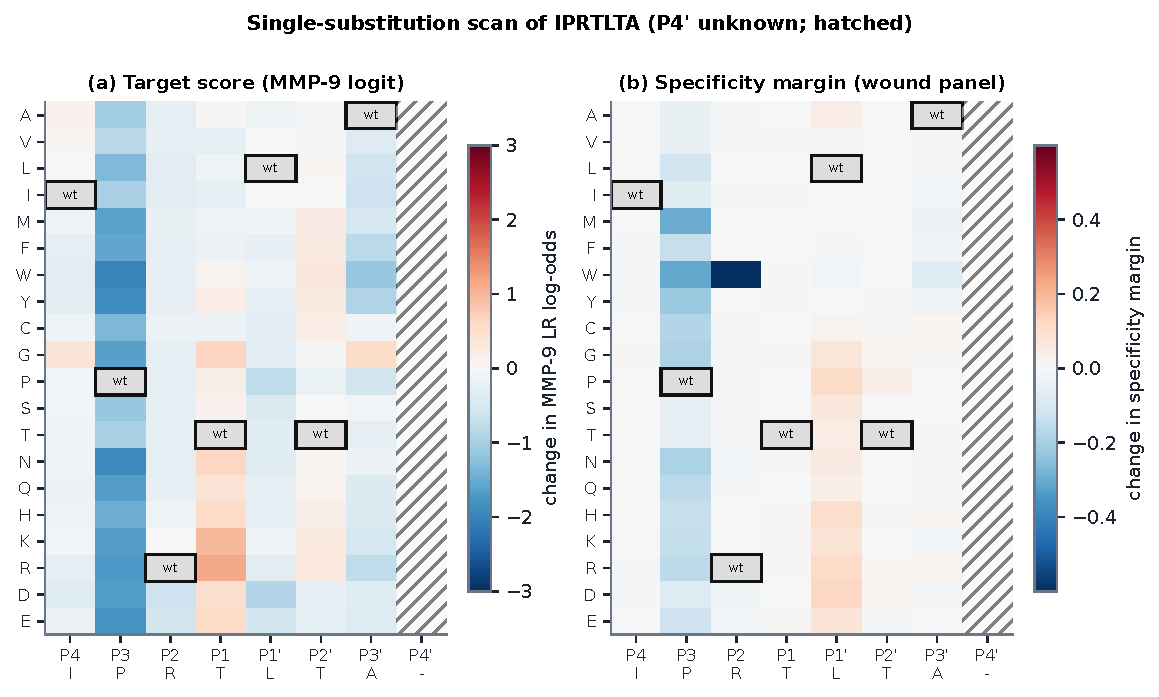
\includegraphics[width=\textwidth]{../figures/F18_mutation_scan.pdf}
  \caption{Single-substitution scan of the A11 core. \textbf{A:} change in MMP-9
    logistic-regression log-odds. \textbf{B:} change in specificity margin in the
    wound panel.}
  \label{fig:scan}
\end{figure}

\subsection{Result: the interactive tool}

The browser tool embeds the seven models and the five structures and loads the
3Dmol.js renderer from a CDN. Its JavaScript scoring engine was compared with
the Python package on $154$ random and $8$ gapped windows across all seven
proteases: logistic-regression scores, PSSM scores, per-position contributions
and percentiles of full windows agree to about $10^{-15}$, and percentiles of
gapped windows agree within $0.012$, the only difference being the random-number
generator behind the matched null \CONF. The built page was exercised in a
headless browser (no script errors; controls, presets, scan clicks and structure
switching respond; no horizontal overflow at phone width) \CONF.

%=======================================================================
\section{Summary: Confirmed Results, Working Assumptions, and Open Questions}
\label{sec:summary}

\begin{center}
\small\renewcommand{\arraystretch}{1.3}
\begin{tabular}{@{}p{1cm}p{4.6cm}p{8.6cm}l@{}}
\toprule
\textbf{Part} & \textbf{Component} & \textbf{Status} & \\
\midrule
A & Positive windows & Rebuilt from MEROPS, Eckhard and Yang sources; counts reproduce the earlier pipeline; $75$ of $75$ elastin rows verified against UniProt & \CONF \\
A & Removal of synthetic LasB positives & Rule-generated and hand-typed windows removed; LasB uses source windows only & \CONF \\
A & Negatives as true non-substrates & Unlabelled windows assumed negative; contamination bounded but unknown & \FLAG \\
A & LasB positives & $76\%$ from one protein (elastin); model behaves as an elastin-likeness score & \CONF \\
B & VHSE table and labels & Regenerated from the archived source and unit-tested; the earlier table had $35$ of $160$ values wrong & \CONF \\
B & Additive position-specific model & Trees do not exceed additive models by more than $0.007$ AUROC & \CONF \\
B & PSSM smoothing $\beta,\epsilon$ & Fixed, not tuned & \FLAG \\
C & Percentile comparability & Uniform under the null by construction; resolution $10^{-3}$ & \CONF \\
C & Harmonic-mean consensus and max-competitor margin & Reasoned, not validated against a selectivity ground truth & \FLAG \\
D & Detection performance & Cluster-aware AUROC $0.77$ (MMP-9) to $0.95$ (faecal); random and clustered folds differ by at most $0.007$; label-shuffle $0.49$--$0.53$ & \CONF \\
D & Representation choice & VHSE leads below about $200$ positives; PSSM and one-hot lead on MMP-2 and MMP-8; consensus retained & \CONF \\
D & Panel negatives & Improve cross-protease AUROC on every protease at $0.01$--$0.02$ cost against background & \CONF \\
D & Selectivity within the MMPs & Held-out AUROC $0.53$--$0.72$; partly reflects genuine promiscuity in the labels & \CONF \\
E & MMP-9 consensus recovery & Pro at $\pos{3}$ first, Leu/Ile at $\prm{1}$ first and second; Ser/Thr not recovered, as expected from the phage-vector artefact & \CONF \\
E & Structures & Catalytic-site residues derived from coordinates; HEXXHXXGXXH confirmed in three MMPs & \CONF \\
E & Measured kinetics ($n=11$) & Positive rank association (PSSM $\rho=0.70$, logistic regression $0.58$); intervals wide; not corrected for multiplicity & \CONF \\
E & Single-mutant effects & Direction correct for both; Leu to Ala at $\prm{1}$ underestimated & \CONF \\
F & Alignment of sensor cores & Three of four cores corrected to scissile-aware windows; 3-plex condition number $61.7 \to 16.1$ & \CONF \\
F & Optimised candidates & Extrapolate beyond the training distribution & \FLAG \\
F & Prospective wet-lab test & Not yet performed & \FLAG \\
\bottomrule
\end{tabular}
\end{center}

\textbf{Bottom line.} The models discriminate confirmed cleavage windows from
background reliably (cluster-aware AUROC $0.77$ to $0.95$), the result is
robust to near-duplicate leakage and to label shuffling, and the learned
specificity agrees with published MMP-9 specificity and with the active-site
structures of the enzymes. What the models cannot do is equally clear. Selectivity
among the MMPs cannot be obtained from a P4--P4$'$ window, the LasB model reflects
its single-protein source, scores rank resemblance to observed sites and are not
rates, and the external validation ($n=11$) supports direction but not
magnitude. What requires direct experimental attention is a prospective test:
measured relative activities of new peptides across the panel, against which the
percentile margin can be checked.


%=======================================================================
\section*{References}

\begin{enumerate}[label={[\arabic*]},noitemsep,leftmargin=*]
\item Kridel SJ, Chen E, Kotra LP, Howard EW, Mobashery S, Smith JW (2001).
  Substrate hydrolysis by matrix metalloproteinase-9.
  \textit{J Biol Chem} 276(23):20572--20578. \textbf{kridel2001.pdf}
  (papers/layer\_09/)

\item Nagase H, Woessner JF Jr (1999). Matrix metalloproteinases.
  \textit{J Biol Chem} 274(31):21491--21494. \textbf{nagase\_woessner1999.pdf}
  (papers/layer\_00/)

\item Trengove NJ, Stacey MC, MacAuley S, Bennett N, Gibson J, Burslem F,
  Murphy G, Schultz G (1999). Analysis of the acute and chronic wound
  environments: the role of proteases and their inhibitors.
  \textit{Wound Repair Regen} 7:442--452. \textbf{trengove1999.pdf}
  (papers/layer\_00/)

\item Eckhard U, Huesgen PF, Schilling O, Bellac CL, Butler GS, Cox JH, Dufour A,
  Goebeler V, Kappelhoff R, Keller UAD, Klein T, Lange PF, Marino G, Morrison CJ,
  Prudova A, Rodriguez D, Starr AE, Wang Y, Overall CM (2016). Active site
  specificity profiling of the matrix metalloproteinase family: proteomic
  identification of 4300 cleavage sites by nine MMPs explored with structural and
  synthetic peptide cleavage analyses. \textit{Matrix Biol} 49:37--60.
  \textbf{1-s2.0-S0945053X15001298-mmc4.xlsx, -mmc5.xlsx}
  (substrate\_predictor/data/raw/eckhard2016/)

\item Yang J, Zhao HL, Ran LY, Li CY, Zhang XY, Su HN, Shi M, Zhou BC, Chen XL,
  Zhang YZ (2015). Mechanistic insights into elastin degradation by pseudolysin,
  the major virulence factor of the opportunistic pathogen \textit{Pseudomonas
  aeruginosa}. \textit{Sci Rep} 5:9936. \textbf{srep09936-s1.pdf}
  (substrate\_predictor/data/raw/yang2015/)

\item Mei H, Liao ZH, Zhou Y, Li SZ (2005). A new set of amino acid descriptors
  and its application in peptide QSARs. \textit{Biopolymers} 80(6):775--786.
  Descriptor definition checked against the published abstract; values archived
  as \textbf{vhse8\_table\_peptides\_0.5.0.json} (substrate\_predictor/references/)

\item Henikoff S, Henikoff JG (1992). Amino acid substitution matrices from
  protein blocks. \textit{Proc Natl Acad Sci USA} 89:10915--10919. Matrix values
  archived as \textbf{blosum62\_biopython.json} (substrate\_predictor/references/)

\item MEROPS peptidase database, \texttt{Substrate\_search} and peptidase-unit
  records. \textbf{Substrate\_search.txt} (cross\_reactivity\_matrix/data/raw/)

\item UniProtKB/Swiss-Prot release 2026\_03, amino-acid composition (Expasy
  release statistics, section 6.1) and sequence P04985.
  \textbf{swissprot\_composition\_2026\_03.json} (substrate\_predictor/references/)

\item RCSB Protein Data Bank entries 1GKC, 1QIB, 1JAN, 1HNE and 1EZM.
  \textbf{MMP9.pdb, MMP2.pdb, MMP8.pdb, NE.pdb, LASB.pdb}
  (substrate\_predictor/data/structures/processed/)

\end{enumerate}

\end{document}
